\chapter{THIẾT KẾ VÀ HIỆN THỰC HỆ THỐNG}

\section{Sơ đồ thiết kế hệ thống}

Sơ đồ thiết kế của hệ thống điều khiển cánh tay robot Denso được trình bày ở hình dưới:

\begin{figure}[H]
    \centering
    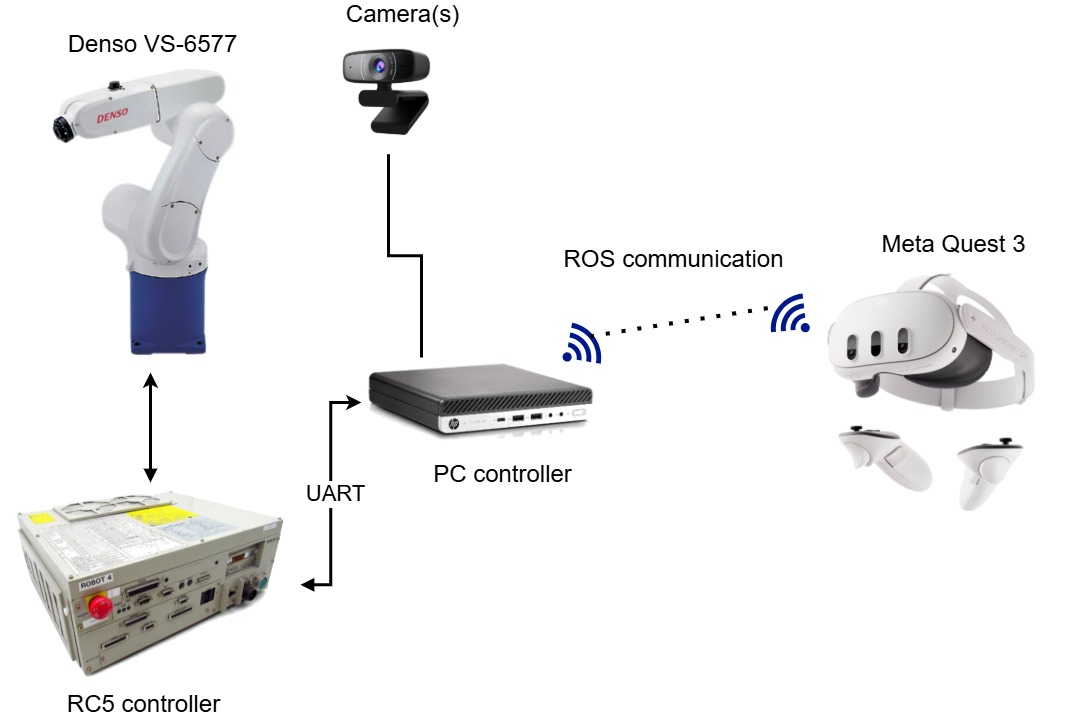
\includegraphics[width=1\linewidth]{Images/Implementation/System_architecture.jpg}
    \caption{Sơ đồ thiết kế của hệ thống điều khiển}
    \label{fig:placeholder}
\end{figure}

Trong sơ đồ này, có các khối chức năng chính có thể kể đến như:

\begin{itemize}
    \item \textbf{Cánh tay robot Denso VS-6577E}: 
    
    Đây là thiết bị điều khiển chính trong dự án, với 6 trục tự do, cánh tay có độ linh hoạt và ổn định cao, phù hợp cho các công việc đòi hỏi sự chỉnh xác, kể cả trong môi trường công nghiệp
    \item \textbf{Máy điều khiển RC5}:

    Đây là một máy điều khiển robot hiệu năng cao, RC5 đóng vai trò quan trọng để trực tiếp điều khiển các trục của cánh tay robot Denso thông qua các dây kết nối ở cổng CN12. Điều này cũng đồng nghĩa là để có thể xoay các trục cánh tay, ta cần phải tận dụng RC5. Như đã trình bày ở Chương 2, ngoài khả năng điều khiển trực tiếp bằng teach pendant, RC5 cũng cho phép người dùng viết "PAC script" - là một ngôn ngữ lập trình chuyên biệt cho thiết bị để điều khiển từ nhà sản xuất Denso. Qua việc thiết kế các PAC script, nhóm hiện thực khả năng nhận lệnh điều khiển cánh tay robot thông qua lệnh UART, đẩy các tính năng chính và lớn lên module tiếp theo: PC Controller.
    \item \textbf{PC Controller}: 

    PC Controller đóng vai trò là bộ điều khiển trung tâm, là cầu nối giữa thiết bị điều khiển thông dụng khác với cụm RC5-Cánh tay VS-6577E. Trên PC Controller sẽ được tập trung phát triển các cơ chế điều khiển cánh tay cũng như cập nhật trạng thái cánh tay tận dụng ROS2. ROS2 đem lại cho nhà phát triển một hệ sinh thái đa dạng, mạnh mẽ, giúp nhà phát triển có thể dễ dàng triển khai các ứng dụng robot đa dạng, phức tạp mà không bị phụ thuộc bởi máy RC5 của Denso. Nhóm tập trung xây dựng một cơ chế giao tiếp hiệu quả, tốc độ cao và đáng tin cậy giữa thiết bị điều khiển bên ngoài và cánh tay robot Denso, từ đó tạo nền móng cho việc phát triển nhiều ứng dụng trên cánh tay robot sau này.

    \item \textbf{Các camera}:

    Như đã trình bày ở các phần trên và quan sát cả các nghiên cứu liên quan, Camera là một thành phần không thể thiếu trong kiến trúc hệ thống, với vai trò quan trọng là mang lại phản hồi hình ảnh thực tế về môi trường xung quanh và chính cánh tay robot được điều khiển ở xa, qua đó tăng cường trải nghiệm vận hành, điều khiển, giúp tăng hiệu suất điều khiển từ xa hơn so với các phương pháp truyền thống.

    \item \textbf{Meta Quest 3}

    Meta Quest 3 được nhóm lựa chọn là thiết bị VR sẽ được sử dụng trong đồ án. Một ứng dụng VR sẽ được phát triển tận dụng Unity Engine và thư viện VR được cung cấp và phát triển bởi Meta, với mục tiêu xây dựng ứng dụng điều khiển, tương tác hiệu quả, trực quan, đồng bộ tốt với cánh tay thực tế. Việc cho phép người dùng sử dụng VR để điều khiển cánh tay sẽ đem lại trải nghiệm sinh động, trực quan, tăng hiệu quả điều khiển cho người dùng từ xa mà không đánh đổi sự tiện lợi, cung cấp đầy đủ các tính năng điều khiển thông dụng như trên thiết bị truyền thống.
\end{itemize}

Các phần tiếp theo lần lượt trình bày phương thức hiện thực các module chính đã được mô tả phía trên.

\section{Xây dựng chương trình điều khiển cánh tay bằng RC5}

\subsection{Thiết kế chương trình}

Trong giai đoạn một, chương trình trên RC5 dù đơn giản, nhưng lại có nhiều điểm yếu như sau:
\begin{itemize}
    \item Chương trình phụ thuộc vào hàm nhận và tách dữ liệu UART tự động của RC5, tuy nhiên hàm lại không hỗ trợ cơ chế nhận diện và xử lý khi chuỗi nhận bị lỗi. Khi bị lỗi, chương trình bị dừng hoàn toàn và phải khởi động lại một cách thủ công
    \item Chu trình hoạt động không liên tục: Luồng chạy yêu cầu phải nhận dữ liệu, xử lý, xong mới xoay cánh tay robot. Điều này tạo ra điểm ngắt quãng giữa các lệnh xoay, khiến cho robot xoay bị giật và không mượt mà
    \item Hàm xoay robot "Move" tốn nhiều thời gian tính toán thay vì dùng các lệnh xoay trực tiếp trục như "DriveA"
\end{itemize}

Ở giai đoạn này, chương trình đã được nâng cấp đáng kế để giải quyết hai điểm yếu lớn trên, cụ thể:

\begin{itemize}
    \item Phân tách chương trình gốc thành 4 chương trình con khác nhau, mỗi chương trình đảm nhiệm một nhiệm vụ cụ thể:
    \begin{itemize}
        \item \lstinline[style=inlinecode]{GET_JOINT.pac}: Đọc giá trị các trục hiện tại của Robot và gửi giá trị đó qua UART
        \item \lstinline[style=inlinecode]{task0.pac}: Đọc lệnh UART từ PC Controller gửi xuống và lưu vào buffer.
        \item \lstinline[style=inlinecode]{TASK1CRC.pac}: Khi có giá trị buffer mới, tiến hành xử lý dữ liệu đó dưới dạng string để giải mã lệnh điều khiển, và lưu vào một Ring Buffer
        \item \lstinline[style=inlinecode]{task3.pac}: Đọc lệnh điều khiển từ Ring Buffer và xoay cánh tay robot tương ứng
    \end{itemize}
    \item Sử dụng cơ chế chạy đồng thời: ngôn ngữ PAC trên RC5 cho phép chạy các đoạn chương trình một cách đồng thời theo chu kì thời gian định trước. 
    \item Viết chương trình riêng để xử lý lệnh UART ở dạng string để có quyền kiểm soát và phát hiện lỗi
    \item Sử dụng hàm xoay từng trục trực tiếp để giảm thiểu thời gian tính toán.
\end{itemize}

Sau cùng, chương trình tổng \lstinline[style=inlinecode]{MAIN.pac} sẽ chạy bốn chương trình trên đồng thời theo chu kì, kèm theo một số khởi tạo cần thiết cho hoạt động của cánh tay robot.

\begin{lstlisting}
'!TITLE "MAIN"
PROGRAM MAIN
    DEFIN li1
    REM ========= I1 notify that new string data is received. after processed, set I1 to 0 to wait for new data.
    I1 = 0
    REM ========= I4 and I5 used for ring buffer for processed joint.
    I4 = 0
    I5 = 0
    FLUSH #1
    FOR li1 = 0 to 99
        J[li1] = (0,0,0,0,0,0)
    NEXT li1
    REM ==== Read Serial Task
    RUN TASK0, C = 10
    DELAY 20
    REM ==== Process recevied data
    RUN TASK1CRC, C = 15
    REM ==== RUN ROBOT
    RUN TASK3, C = 35
    REM ==== Transmit current joint
    RUN GET_JOINT, C = 100
END
\end{lstlisting}

Phần tiếp theo trình bày chi tiết cơ chế hoạt động của chương trình tại RC5.

\subsection{Cơ chế nhận lệnh, xử lý lệnh kiểu chuỗi và xoay cánh tay robot}

Đây chính là cơ chế quan trọng nhất trong chuỗi lệnh điều khiển của RC5, chính vì vậy nó được thiết kế để đảm bảo các tiêu chí: hoạt động ổn định, nhanh, mượt mà và có khả năng chịu lỗi để có thể chạy liên tục trong thời gian dài. Kiến trúc hoạt động của chương trình được thể hiện bên dưới:

\begin{figure}[H]
    \centering
    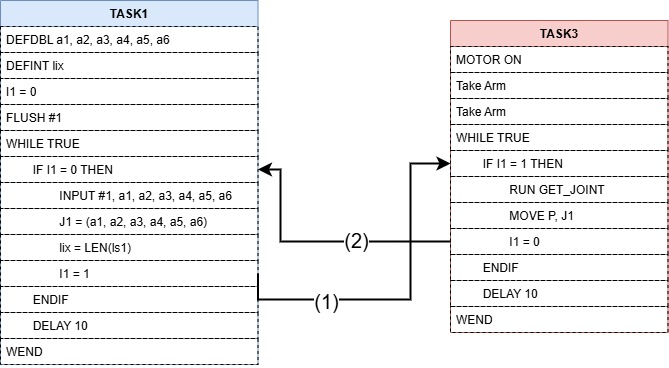
\includegraphics[width=0.8\linewidth]{Images/Implementation/Control/RC5_software.jpg}
    \caption{Kiến trúc chương trình điều khiển RC5}
    \label{fig:rc5-program-architecture}
\end{figure}

Chương trình MAIN.pac có vai trò khởi chạy các chương trình con theo chu kì phù hợp, trong đó:
\begin{itemize}
    \item \textbf{TASK0}: dùng để đọc lệnh Serial, do đó cần chạy liên tục và nhanh với chu kì 10ms. Lệnh UART sẽ được rút ra từ buffer UART nội bộ của máy RC5, chỉ khi có dữ liệu serial và cờ đọc sẵn sàng (\lstinline[style=inlinecode]{I1 = 0}). Dữ liệu UART được đọc và lưu trữ vào biến chuỗi toàn cục \lstinline[style=inlinecode]{S1}, cờ đọc bị chặn (\lstinline[style=inlinecode]{I1 = 1}) để cho phép code xử lý chuỗi bắt đầu chạy ở \textbf{TASK1CRC}
    \item \textbf{TASK1CRC:} Khi cờ \lstinline[style=inlinecode]{I1 = 1}, chương trình xử lý chuỗi sẽ lấy dữ liệu lưu trong \lstinline[style=inlinecode]{S1} và bắt đầu nhiệm vụ phân tách. Format của lệnh điều khiển ở dạng như sau:
    \begin{lstlisting}[language={}]
    J1,J2,J3,J4,J5,J6#LEN_PAYLOAD
\end{lstlisting}
    Trong đó, \lstinline[style=inlinecode]{J[X]} lần lượt là giá trị góc (tính theo độ) của từng trục, giá trị này cần ở dạng số nguyên có dấu. Trên thực tế, robot hoàn toàn có thể được điều khiển với giá trị góc là số thực (có dấu chấm động), tuy nhiên, việc xử lý chuỗi có dấu chấm động tăng tính phức tạp và thời gian chạy của hàm xử lý chuỗi, do đó giá trị góc dạng số thực sẽ sẽ được gửi xuống UART ở dạng \lstinline[style=inlinecode]{angle * 100}, và chia ngược lại ở RC5 

    Ngoài ra, format lệnh còn có thêm \lstinline[style=inlinecode]{LEN_PAYLOAD}, được phân cách bởi ký tự đặc biệt "\#", dùng để chứa độ dài của chuỗi lệnh trước dấu "\#". Lý do là vì trong quá trình phát triển, giao tiếp giữa RC5 và PC controller thường gặp trục trặc, chủ yếu là do dữ liệu UART truyền tới RC5 bị mất hoặc dư kí tự, từ đó tạo giá trị góc sai lệch hoặc lỗi trong lúc giải mã chuỗi. Chính vì vậy, việc sử dụng \lstinline[style=inlinecode]{LEN_PAYLOAD} có tác dụng như một cơ chế kiểm tra toàn vẹn dữ liệu đơn giản, giúp chương trình xử lý chuỗi có thể phát hiện sớm chuỗi bị lỗi và loại bỏ, đảm bảo khả năng hoạt động ổn định trong thời gian dài ở phía cánh tay robot. Khối CRC\_check ở sơ đồ trên thể hiện tính năng này, trong đó chuỗi được xem là lỗi khi:
    \begin{enumerate}
        \item Không tìm thấy dấu "\#"
        \item Tìm thấy dấu "\#", nhưng \lstinline[style=inlinecode]{LEN_PAYLOAD} khác với độ dài của chuỗi nhận được bên trái dấu "\#".
    \end{enumerate}

    Chuỗi dữ liệu hợp lệ (pass được khối CRC\_check) sẽ tiến tới phần bóc tách dữ liệu góc joint\_seperation, qua đó từng giá trị số nguyên sẽ được lấy ra, convert sang giá trị số và chia 100 để lấy giá trị số thực của góc xoay. Sáu giá trị góc sau đó lưu vào biến toàn cục \lstinline[style=inlinecode]{J[I5]}. \lstinline[style=inlinecode]{I5 + 1} và \lstinline[style=inlinecode]{I1 = 0} để cho phép \textbf{TASK0} đọc vào chuỗi UART tiếp theo.
    \item \textbf{TASK3:} Chương trình được cải tiến để tránh khoảng ngừng giữa các lần xoay bằng cơ chế Ring Buffer. Cụ thể, trong RC5 cho phép người dùng sử dụng các biến toàn cục, trong đó \lstinline[style=inlinecode]{J[X]}, với X từ 0 -> 99 là 100 biến toàn cục dùng để chứa giá trị góc (joint). Hai biến toàn cục \lstinline[style=inlinecode]{I4, I5} được sử dụng, trong đó 
    \begin{enumerate}
        \item \lstinline[style=inlinecode]{I5} thể hiện lệnh xoay joint \textbf{trong tương lại}, liên tục tăng mỗi khi chuỗi được xử lý xong ở \textbf{TASK1CRC} và giá trị góc được lưu vào \lstinline[style=inlinecode]{J[I5]}
        \item Ở \textbf{TASK3}, \lstinline[style=inlinecode]{I4} thể hiện lệnh xoay joint \textbf{đã xử lý}, nếu \lstinline[style=inlinecode]{I4 < I5} tức là vẫn còn lệnh chưa được xử lý, \lstinline[style=inlinecode]{J[I4]} sẽ được dùng để xoay các trục robot, sau đó tăng \lstinline[style=inlinecode]{I4 + 1} cho tới khi đuổi kịp \lstinline[style=inlinecode]{I5}
    \end{enumerate}
    Cơ chế này đem lại sự linh hoạt và giảm đáng kể các khoảng ngừng giữa các lệnh xoay, bởi I5 thì cứ tăng (chuỗi được xử lý liên tục), trong khi ở \textbf{TASK3}, I4 cũng liên tục đuổi theo I5 và xoay các trục của cánh tay theo chuỗi lệnh. I5 chắc chắn sẽ chạy nhanh hơn I4, nên \textbf{TASK3} cũng sẽ liên tục có các giá trị góc xoay mới mà không bị ngắt giữa chừng.
\end{itemize}

\subsection{Cơ chế cập nhật trạng thái robot}

So với cơ chế điều khiển, cơ chế cập nhật trạng thái của robot có phần đơn giản hơn hơn nhờ sự hỗ trợ trực tiếp từ RC5. Chương trình \textbf{GET\_JOINT} liên tục lấy giá trị góc của 6 trục robot thông qua \lstinline[style=inlinecode]{CURJNT} và gửi lên PC Controller mỗi 100ms với format:

\begin{lstlisting}[language={}]
    j1, j2, j3, j4, j5, j6\r
\end{lstlisting}

So với lệnh điều khiển, lệnh cập nhật trạng thái có phần ổn định và ít lỗi hơn, do đó cơ chế CRC hiện chưa cần thiết. Thêm nữa, ở phía PC controller đã có nhiều đoạn code xử lý và phát hiện lỗi ở nhiều cấp độ: cấp UART, cấp Driver và cấp Hardware Interface, đủ để loại bỏ các chuỗi trạng thái lỗi mà vẫn đảm bảo chương trình hoạt động ổn định trong thời gian dài.

\section{Kiến trúc phần mềm điều khiển bằng ROS2}

Kèm theo với nhiều cải tiến trong code xử lý lệnh ở RC5, độ ổn định giữa giao tiếp RC5 - PC controller tạo tiền đề để phát triển, mở rộng hơn kiến trúc phần mềm ROS2 đã có ở giai đoạn một. Tiêu chí thiết kế vẫn tương tự ở giai đoạn hai, phần hiện thực sẽ trở nên phức tạp hơn đối với tầng điều khiển ở PC Controller. ROS2 được sử dụng làm nền tảng để xây dựng cơ chế điều khiển robot, với nhiều công cụ hỗ trợ và mạnh mẽ nhằm tăng tốc khả năng hiện thực. Hơn nữa, đề tài chủ trương xây dựng chương trình Ros2 sử dụng ngôn ngữ C++ thay vì python và ROS1, với mục tiêu là sử dụng những công nghệ mới nhất trong lập trình robot, cũng như tạo cơ hội để tiếp cận những bộ công cụ hiện đại hơn. Về phiên bản ROS2, đề tài sử dụng ROS2 Humble trong Ubuntu 22.04, do sự phổ biến của nó trong cộng đồng phát triển cũng như được hỗ trợ rộng rãi bởi nhiều bộ công cụ bên thứ ba. Kết hợp với ROS2, đề tài sử dụng thêm Ros2-Control và ROS2-Moveit, nhanh chóng tạo dựng cơ chế điều khiển cánh tay robot theo tiêu chuẩn của những dự án ROS2 đã được xây dựng và nghiên cứu trước đó.

Hiện thực ROS2 của đồ án có thể tìm thấy ở đây: \href{https://github.com/ngoccatt/ros2_arctos_HCMUT}{ros2\_arctos\_HCMUT}

\subsection{Sơ đồ kiến trúc phần mềm dựa trên Ros2-Control}

\begin{figure}[H]
    \centering
    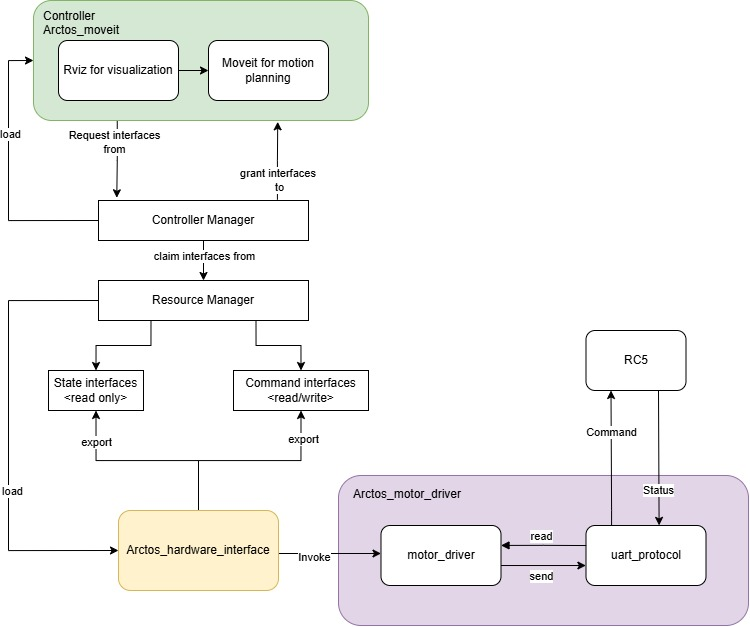
\includegraphics[width=0.8\linewidth]{Images/Implementation/Control/ros2_control.jpg}
    \caption{Sơ đồ kiến trúc phần mềm dựa trên Ros2-Control}
    \label{fig:placeholder}
\end{figure}

Đề tài chủ trương xây dựng chương trình điều khiển cánh tay robot VS-6577E theo kiến trúc của Ros2-Control, bao gồm các khối như controller, hardware interface và driver. Xây dựng phần mềm theo kiến trúc của Ros2-Control đem lại những ưu điểm như

\begin{itemize}
    \item Module hóa các lớp điều khiển, giúp dễ kiểm soát, bảo trì và kiểm thử.
    \item Tạo khả năng mở rộng và dùng lại tốt, có thể dễ dàng điều chỉnh để thay thế phần driver hoặc hardware interface sử dụng cho robot khác, trong khi phần controller và lớp ứng dụng cao hơn được giữ nguyên.
    \item ROS2-Control sử dụng cơ chế hoạt động theo chu kì \textbf{update-write-read} đơn giản nhưng mạnh mẽ, là nền tảng để xây dựng chương trình vận hành robot thời gian thực
    \item Tích hợp dễ dàng với MoveIt để xử lý việc điều khiển và lập kế hoạch quỹ đạo cánh tay với các giải thuật động học hiệu quả
\end{itemize}

Phần tiếp theo mô tả các khối chính trong mô hình kiến trúc theo Ros2-control mà đề tài vận dụng.

\subsection{Khối Driver}

Khối Driver là tầng dưới cùng trong kiến trúc Ros2-Control, có vai trò giao tiếp trực tiếp với phần cứng - cánh tay robot VS-6577E thông qua máy điều khiển RC5 và tay gắp Gripper-A thông qua Driver-Hat-A. Cả hai bộ điều khiển trung gian: RC5 và Driver-Hat-A đều hỗ trợ giao thức UART, do đó khối \lstinline[style=inlinecode]{UartProtocol} có thể được tái sử dụng ở cả hai phía. Tuy nhiên, mỗi driver sẽ khởi tạo một đối tượng \lstinline[style=inlinecode]{UartProtocol} riêng để đảm bảo quá trình truyền nhận dữ liệu tách biệt và không xung đột.

\subsubsection{Khối UartProtocol} 

Khối UartProtocol được xây dựng các chức năng để hỗ trợ truyền/nhận dữ liệu UART, phân tích dữ liệu theo định dạng đã đề xuất và lưu trữ dữ liệu nhận được để tránh mất gói tin. Một số tính năng của module này có thể kể tới như:
\begin{itemize}
    \item \textbf{Thiết kế class}: Uart\_protocol có thể được khởi tạo như một object riêng biệt ở mỗi module khác cần sử dụng, giúp tách biệt luồng dữ liệu và tránh xung đột khi tạo nhiều giao tiếp UART.
    
    \item \textbf{Cơ chế lưu dữ liệu nhanh chóng}: Khi có dữ liệu mới, module này sẽ nhanh chóng lưu nó vào một buffer riêng, và khi cần sẽ lấy dữ liệu ra theo FIFO. Để đáp ứng cơ chế này, module sử dụng UART cần gọi hàm \lstinline[style=inlinecode]{readToBuffer()} liên tục trong một thread riêng, và gọi \lstinline[style=inlinecode]{getFromBuffer()} để lôi dữ liệu ra ngoài khi cần.
    
    \item \textbf{Hàm hỗ trợ truyền dữ liệu cơ bản}: hai hàm \lstinline[style=inlinecode]{sendMsg()} và \lstinline[style=inlinecode]{sendMsgWithCLRF()} có thể được sử dụng để truyền một chuỗi kí tự đi tới kết nối UART.
    
    \item \textbf{Hỗ trợ riêng cho giao tiếp với RC5}: hai hàm \lstinline[style=inlinecode]{sendPosition()} và \lstinline[style=inlinecode]{decodeMessage()} hỗ trợ cách thức đơn giản hơn để truyền lệnh (có bao gồm cơ chế crc theo chiều dài chuỗi) và giải mã giá trị trục thực tế của robot.
    
\end{itemize}

\subsubsection{Motor Driver}

Phần Motor Driver được xây dựng để quản lý trạng thái và điều khiển các trục của cánh tay robot VS-6577. Module Motor driver mang đặc trưng điều khiển cụ thể, phù hợp với RC5 và VS-6577. Điểm mạnh của module này là: 
\begin{enumerate}
    \item Cung cấp khả năng quản lý các trục xoay bằng nhiều thuộc tính như tên trục, giới hạn min/max trục, góc xoay hiện tại, góc xoay yêu cầu, feedback, thời gian cập nhật/điều khiển...
    \item Cung cấp cơ chế kiểm tra nhiều lớp tính hợp lệ của dữ liệu điều khiển cũng như giá trị trạng thái trục được gửi lên từ cánh tay robot thực tế.
    \item Tiết kiệm thời gian xử lý bằng cách kiểm tra tính mới của giá trị trạng thái trước khi giải mã và xử lý.
    \item Thiết kế để dễ dàng quản lý, mở rộng và có thể áp dụng để điều khiển với số lượng trục linh động, các hàm được xây dựng phụ thuộc vào tham số mà người dùng hoàn toàn có thể điều chỉnh ở file config mà không cần phải build lại phần mềm.
\end{enumerate}

Cách thiết kế của Motor Driver cho phép mỗi trục là một đối tượng riêng biệt (\lstinline[style=inlinecode]{JointConfig}), giúp dễ dàng quản lý trạng thái và thuộc tính hiệu quả. Khi có lệnh mới, giá trị góc xoay yêu cầu được lưu ngay vào đối tượng \lstinline[style=inlinecode]{JointConfig}. Khi cần gửi dữ liệu điều khiển xuống RC5, các giá trị góc xoay yêu cầu được thu thập từ mỗi đối tượng và tạo thành một chuỗi lệnh ở dạng sau, với sự hỗ trợ của module Uart:

\begin{lstlisting}
J1,J2,J3,J4,J5,J6#LEN_PAYLOAD
\end{lstlisting}

Ngược lại, dữ liệu trạng thái trục truyền lên từ RC5 được phân tách, kiểm tra tính hợp lệ của dữ liệu và lưu ngược lại trong \lstinline[style=inlinecode]{JointConfig} tương ứng.

\subsubsection{Servo Driver}

Khối Servo Driver được thiết kế dựa trên Motor Driver, tuy nhiên được tinh gọn hơn là chỉ dùng để gửi lệnh tới một Servo. Mục tiêu của module này là giao tiếp với Driver-Hat-A để điều khiển tay gắp Gripper-A, và hiện Driver-Hat-A cũng chỉ hỗ trợ điều khiển một servo duy nhất, nên Servo Driver chỉ đặt thêm một ràng buộc không cho tạo nhiều hơn 1 đối tượng \lstinline[style=inlinecode]{JointConfig}. Một lý do nữa cần phải phân tách ra so với khối Motor Driver, đó là giao tiếp với Driver-Hat-A có format quy định tương đối khác so với RC5. Cụ thể, lệnh cần được gửi ở dạng JSON format. Đề tài sử dụng thư viện \href{https://github.com/nlohmann/json}{JSON for Modern C++} để có thể nhanh chóng tạo và xử lý chuỗi ở dạng JSON. Lệnh điều khiển có dạng như sau:

\begin{lstlisting}[language=json]
{"T":121,"angle":0.67,"spd":100,"acc":10}
\end{lstlisting}

Trong đó "T":121 ám chỉ đây là lệnh điều khiển, (angle) là giá trị góc xoay (radian) mà servo cần đạt tới để đóng hay mở tay gắp, với tốc độ (spd) từ 0 -> 4096 và gia tốc (acc) từ 0 -> 254. Giá trị 0 ở spd và acc yêu cầu xoay với tốc độ cao nhất.

Để lấy trạng thái góc xoay hiện tại của gripper, ta cần phải gửi lệnh JSON xuống thiết bị, thay vì thiết bị gửi trạng thái liên tục. Định dạng của lệnh là:

\begin{lstlisting}[language=json]
{"T":105}
\end{lstlisting}

Driver-hat-A sẽ phản hồi lại góc xoay, cùng nhiều thông tin khác của tay gắp ở dạng:

\begin{lstlisting}[language=json]
{"T":1051,"pos":3138,"speed":0,"load":-104,"voltage":124,"current":4,"temper":45,"mode":0}
\end{lstlisting}

Trong đó, thông tin về góc xoay hiện tại (pos) được chú trọng, tuy nhiên đây không hẳn là giá trị góc ở đơn vị "độ", mà nó là vị trí của step encoder. Ta cần phải thực hiện tính toán sau để chuyển sang giá trị độ:

\begin{align*}
angle\_deg = (pos - 1024) * (360/4096)
\end{align*}

Thêm nữa, trong quá trình xoay, lệnh đọc trạng thái có thể gửi tới Driver-Hat-A và được phản hồi ngay vị trí hiện tại của servo, cho phép module cao hơn theo dõi trạng thái xoay và góc xoay thực tế của tay gắp.

\subsection{Robot description}

Khi xây dựng ứng dụng điều khiển robot với ROS2, robot description là một module không thể thiếu. Một thư mục Robot Description thường chứa file URDF (Unified Robot Description format), dùng để định nghĩa chi tiết về cấu trúc của robot trong không gian 3D, bao gồm việc nối các bộ phận từ Mesh (một file mô tả hình dáng của cánh tay) lại với nhau và định nghĩa sự liên kết của các bộ phận đó.

Với mục tiêu mô phỏng cánh tay robot một cách chính xác nhất, đề tài chủ trương lấy chính xác mô hình 3D cùng phiên bản của cánh tay VS-6577 từ nhà sản xuất Denso. Mô hình này được import vào phần mềm SOLIDWORK 2024, sau đó thông qua plugin \href{https://github.com/ros/solidworks_urdf_exporter}{\textbf{Solidworks Urdf Exporter}} để export đặc tả URDF của cánh tay cùng các file mesh cấu thành cánh tay robot. Phần tay gắp cũng được nhóm nối trực tiếp vào trục end-effector của cánh tay, cấu thành mô hình 3D cuối cùng đang được đề tài sử dụng. 

\begin{figure}[H]
    \centering
    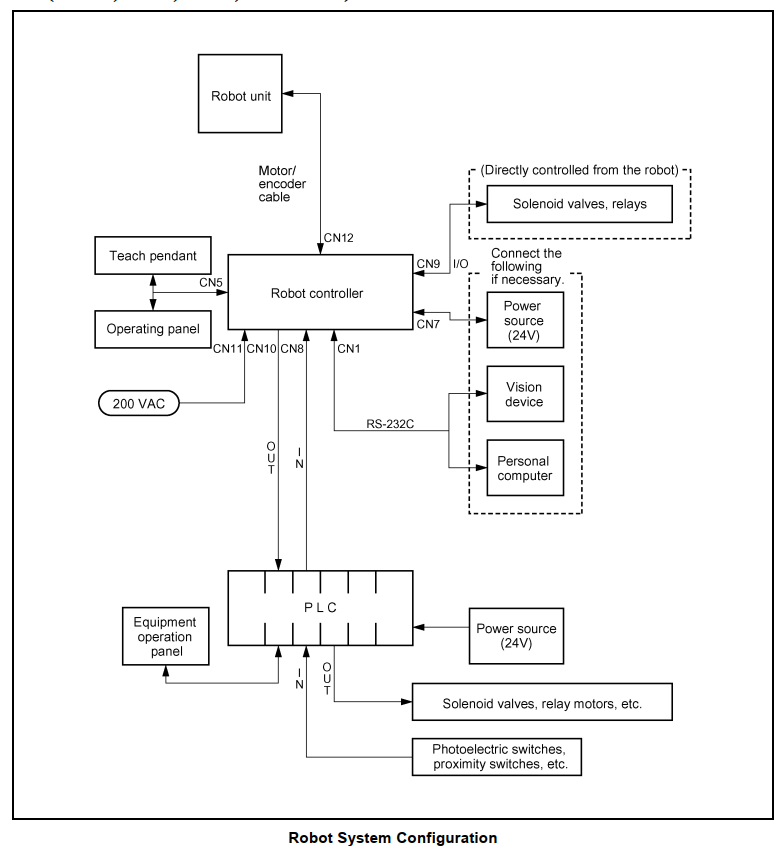
\includegraphics[width=0.85\linewidth]{Images/Implementation/Control/rc5_connection.png}
    \caption{Minh họa kết nối phần cứng phục vụ quá trình tích hợp mô hình robot}
    \label{fig:hw-connection-for-integration}
\end{figure}

Do nội dung file URDF tương đối lớn và nhiều, đề tài thực hiện phân tách thành các file ".xacro" nhỏ hơn. Xacro, hay XML Macros, là một định dạng file được dùng rộng rãi trong ROS2, cho phép lập trình viên tạo những khối đặc tả robot có thể tái sử dụng, đơn giản hóa file URDF thông qua các macro. Đặc tả robot đóng vai trò quan trọng trong việc khởi chạy Ros2-control cũng như MoveIt2, bởi các thông tin này sẽ được boardcast cho toàn mạng ROS2 và được sử dụng triệt để bởi các module để hỗ trợ việc điều khiển hiệu quả, chính xác.

\subsection{Hardware Interface}

Hardware interface là module ở tầng thứ hai trong kiến trúc Ros2-Control, có vai trò làm cầu nối trung gian giữa phần \textbf{Controller} và \textbf{Driver}. Hardware interface sẽ cung cấp các \textbf{command interface} để Controller có thể điều khiển, và \textbf{state interfaces} để cập nhật trạng thái của thiết bị thực từ Driver lên cho Controller, tuân theo thiết kế phần mềm được quy định trong Ros2-Control đối với thành phần Hardware interface. Với việc điều khiển hai thiết bị khác nhau: cánh tay VS-6577 thông qua RC5 và Gripper-A thông qua Driver-Hat-A, hệ thống cần hai hardware interface riêng biệt do cách thức hoạt động khác nhau. Trong phần hiện thực, hai lớp chính được dùng là \lstinline[style=inlinecode]{DensoInterface} cho cánh tay robot và \lstinline[style=inlinecode]{DensoHandInterface} cho tay gắp.

\subsubsection{Quá trình khởi động Hardware Interface}

Theo quy định của Ros2-Control, mọi hardware interface cần được khởi động theo một chu trình cố định, ở từng bước sẽ làm những công việc khởi tạo khác nhau để chuẩn bị kết nối với phần cứng cần điều khiển.

Sơ đồ khởi chạy của Hardware Interface được trình bày như hình dưới:

\begin{figure}[H]
    \centering
    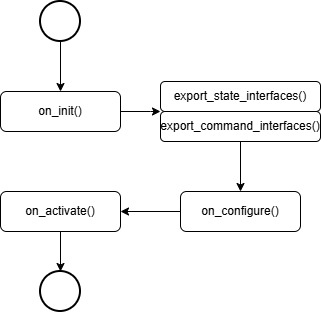
\includegraphics[width=0.5\linewidth]{Images/Implementation/Control/Init_sequence.jpg}
    \caption{Luồng khởi động của Hardware Interface}
    \label{fig:placeholder}
\end{figure}

Luồng khởi động này tuân theo tiêu chuẩn đặt ra bởi Ros2-Control, gồm bốn bước: init, export, configure và activate.

\textbf{on\_init()}

"init" là bước đầu tiên trong luồng khởi tạo. Trong bước này, dữ liệu liên quan tới cánh tay được đặc tả trong Robot Description (file urdf) dưới tag \lstinline[style=inlinecode]{<ros2_control>} sẽ được truyền vào như một tham số của hàm, hỗ trợ trong việc cung cấp thông tin khởi tạo. Một điều lưu ý là tag \lstinline[style=inlinecode]{<ros2_control>} cần chỉ rõ ở tag \lstinline[style=inlinecode]{<hardware>/<plugin>} hardware interface mà nó cần sử dụng, qua đó giúp bản thân Ros2\_Control dẫn các dữ liệu về trục hoặc param tới hardware interface tương ứng. Nhờ cơ chế này, hàm \lstinline[style=inlinecode]{on_init()}  biết được số lượng trục cánh tay robot được mô tả qua dưới tag \lstinline[style=inlinecode]{<ros2_control>}, qua đó tạo dựng các mảng dữ liệu (dạng \lstinline[style=inlinecode]{<vector>} để lưu trữ trạng thái và lệnh điều khiển. Ngoài ra, hàm \lstinline[style=inlinecode]{on_init()} cũng khai báo một số ros parameter mới như \lstinline[style=inlinecode]{motor_id, hardware_type, gear_ratio, inverted, inverted_feedback} ... để chuẩn bị cho bước \lstinline[style=inlinecode]{configure} tiếp theo.

\textbf{export\_state\_interfaces() và export\_command\_interfaces()}

Tiếp đến là bước "export" các "State interface" (dùng để cập nhật trạng thái) và "Command interface" (dùng để ghi lệnh điều khiển). Bước này có vai trò quan trọng trong cấu trúc Ros2-Control, cung cấp đủ interface cho trạng thái và điều khiển thiết bị cho Resource Manager (quản lý tài nguyên), qua đó các Controller có thể "chiếm" những interface này thông qua Controller Manager. Để tránh xung đột về việc sử dụng tài nguyên, một Command interface chỉ có thể được sở hữu bởi một controller, trong khi đó State interface có thể được sử dụng bởi nhiều controller khác nhau. 

Bước này cần đảm bảo các state\_interfaces và command\_interfaces được export đầy đủ như đã khai báo ở dưới tag \lstinline[style=inlinecode]{<ros2_control>}. Nếu export thiếu sẽ khiến cho code bị treo lúc khởi chạy do thiếu interface.

Đối với DensoInterface, các interface sau sẽ được export và sử dụng trong các phương thức read/write:
\begin{itemize}
    \item State interface: \lstinline[style=inlinecode]{joint_position_[i]}, với i là thứ tự của từng trục, đếm từ 0
    \item Command interface: \lstinline[style=inlinecode]{joint_position_command_[i]}, với i là thứ tự của từng trục, đếm từ 0
\end{itemize}

Với DensoHandInterface, các interface sau sẽ được export:
\begin{itemize}
    \item State interface: \lstinline[style=inlinecode]{servo_position_[i]} và \lstinline[style=inlinecode]{servo_velocity_[i]}, tuy nhiên velocity chỉ khai báo chứ không sử dụng, để phù hợp với yêu cầu của GripperActionController. 
    \item Command interface: \lstinline[style=inlinecode]{servo_position_command_[i]}.
\end{itemize}


\textbf{on\_configure()}

Bước "configure" thường được sử dụng để khởi tạo kết nối với phần cứng. Ở bước này, hàm thực hiện đọc các giá trị cấu hình và dùng chúng để khởi tạo Motor/Servo để quản lý cũng như điều khiển thông qua các driver ở lớp dưới. Các giá trị cấu hình này được ghi trong file yaml như ros\_\_parameters, cho phép cấu hình những thông số như ID của motor/servo, vị trí min/max, vị trí 0, vận tốc, gia tốc... Điều này mang lại sự tiện lợi cho việc thay đổi hoạt động của chương trình chỉ bằng cách thay giá trị cấu hình mà không cần build lại phần mềm.

Ví dụ về cấu hình cho 1 trục của \lstinline[style=inlinecode]{arctos_hardware_interface} và DensoHandInterface như bên dưới:

\begin{lstlisting}[language=yaml]
arctos_hardware_interface:
  ros__parameters:
    motors:
      X_joint:
        motor_id: 1
        inverted: false           
        inverted_feedback: false 
        gear_ratio: 1.0
        zero_position: 0.0
        lower_limit: -170.0     
        upper_limit: 170.0      
      ...

denso_hand_interface:
  ros__parameters: 
    gripper:
      gripper_gear_right_joint:
        motor_id: 7
        requires_homing: false
        inverted: false                 
        inverted_feedback: false        
        gear_ratio: 1.0
        zero_position: 0.430
        lower_limit: 0.425             
        upper_limit: 84.9983           
        velocity: 200.0 
        acceleration: 20.0
\end{lstlisting}

Sau khi khởi tạo Motor/servo thông qua bộ driver tương ứng, hàm cũng đảm nhiệm tạo kết nối UART với địa chỉ device, baud\_rate tuỳ chỉnh 

\textbf{on\_activate()}

Sau ba bước trên, Hardware Interface đã khởi tạo và cấu hình đầy đủ thông tin về cánh tay robot, các trục xoay, giới hạn trục, hướng xoay... cũng như tạo kết nối UART. Tới bước này, Hardware Interface sẽ tạo yêu cầu tới cánh tay xoay về vị trí gốc, bằng cách ghi vào \lstinline[style=inlinecode]{joint_position_command_[i]} của mỗi trục = 0, cùng lúc tạo một luồng (thread) song song cho việc lắng nghe dữ liệu truyền vào thông qua UART, lưu nó vào buffer thông qua hàm \lstinline[style=inlinecode]{readToBuffer} của module Kết nối Uart. Với việc sử dụng một luồng riêng để đọc dữ liệu liên tục, Hardware interface đảm bảo mọi dữ liệu UART sẽ được tiếp nhận, lưu trữ mà không bị mất trong quá trình chạy.

\subsubsection{Luồng điều khiển (Write)}

Sau khi đã khởi tạo thành công, trong suốt quá trình chạy của Hardware Interface, sẽ chỉ có 2 hàm được sử dụng đó là \lstinline[style=inlinecode]{write} và \lstinline[style=inlinecode]{read} được chạy theo chu kì. Trong Ros2-Control, ta luôn có một chu kì gồm ba bước: \textbf{update, write, read} lặp lại liên tục trong suốt thời gian hoạt động, trong đó "write" đóng vai trò ghi dữ liệu điều khiển xuống thiết bị phần cứng, "read" có vai trò đọc dữ liệu phản hồi từ phần cứng để cập nhật trạng thái, và "update" do controller thực hiện, đứng giữa để phân tích dữ liệu trạng thái, dữ liệu điều khiển trước đó để đưa ra dữ liệu điều khiển cho chu kì tiếp theo. Đối với luồng điều khiển Write, sẽ có sự khác biệt tương đối giữa DensoInterface và DensoHandInterface.

\begin{figure}[H]
    \centering
    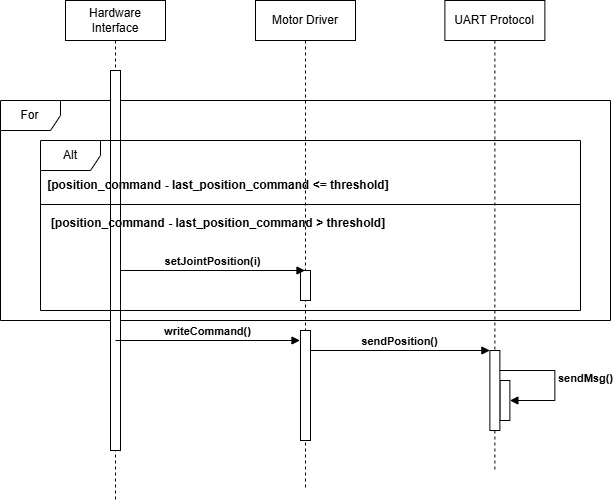
\includegraphics[width=0.8\linewidth]{Images/Implementation/Control/Write_flow.jpg}
    \caption{Luồng điều khiển (Write) của DensoInterface}
    \label{fig:placeholder}
\end{figure}

Đầu tiên, ta sẽ xem xét luồng điều khiển (Write) của DensoInterface. Với mỗi lần tới bước "write" trong chu kì, trước đó "update" đã thực hiên ghi lệnh điều khiển tiếp theo vào "command interface", trong trường hợp này là \lstinline[style=inlinecode]{joint_position_command_[i]}. \lstinline[style=inlinecode]{write} sẽ tiến hành so sánh giữa lệnh điều khiển hiện tại và lệnh điều khiển trước đó có khoảng cách đủ dài (về vị trí) không, tức ta sẽ chỉ cho cánh tay xoay khi sự thay đổi về vị trí (góc xoay) đủ lớn, khi threshold >= 0.001 (rad). Nếu sự thay đổi về vị trí lớn hơn mức ngưỡng 0.001 (rad), hàm \lstinline[style=inlinecode]{setJointPosition()} được gọi với thông tin trục cần xoay và lệnh điều khiển tương ứng với trục đó. Tuy nhiên, trước khi gọi hàm \lstinline[style=inlinecode]{setJointPosition()}, hàm "write" của DensoInterface có thêm cơ chế đặc biệt, gọi là "Trend Learning", với mục tiêu xem xét chuỗi lệnh nhận được có xu hướng tăng hay giảm, và khi phát hiện xu hướng, sẽ cố gắng giữ vững xu hướng đó cho một chuỗi lệnh liên tục tiếp theo. Chức năng này sẽ được bàn luận chi tiết hơn khi trình bày khối MoveIt Servo.

Lưu ý hàm \lstinline[style=inlinecode]{setJointPosition()} chỉ thực hiện việc ghi giá trị điều khiển và lưu giữ giá trị đó cho từng trục vào Motor Driver. Để có thể chính thức sử dụng giá trị lưu giữ, DensoInterface sẽ gọi hàm \lstinline[style=inlinecode]{writeCommand()} từ Motor Driver, Motor Driver sẽ thu thập giá trị điều khiển của 6 trục, đóng gói lại thành một mảng \lstinline[style=inlinecode]{vector<double>}. Sau cùng, hàm \lstinline[style=inlinecode]{sendPosition()} được gọi với giá trị của 6 trục, tạo thành một lệnh điều khiển UART với định dạng phù hợp có thể hiểu được bởi máy RC5, gửi xuống RC5 bằng lệnh \lstinline[style=inlinecode]{sendMsg()}.

% \begin{figure}[H]
%     \centering
%     \includegraphics[width=0.72\linewidth]{Images/Implementation/Control/DensoHand_Write_flow.jpg}
%     \caption{Luồng điều khiển (Write) của DensoHandInterface}
%     \label{fig:denso-hand-write-flow}
% \end{figure}

Đối với DensoHandInterface, cơ chế điều khiển được lược bỏ khối trend learning do nhu cầu điều khiển đơn giản. Hiện tại, Servo Driver sẽ đảm nhận việc chuẩn bị chuỗi JSON hợp lệ để điều khiển, và đoạn chuỗi đó được gửi tới Driver-Hat-A với hàm \lstinline[style=inlinecode]{sendMsgWithCLRF()} của UartProtocol. Trong tương lai, đề tài sẽ chuyển việc chuẩn bị chuỗi điều khiển hợp lệ từ UartProtocol lên khối Motor Driver của DensoInterface, để phần UartProtocol chỉ cung cấp những API cơ bản nhất cho truyền nhận. Điều này sẽ giúp tạo nên sự nhất quán trong cách thiết kế của chương trình.

\subsubsection{Luồng đọc (Read)}

\begin{figure}[H]
    \centering
    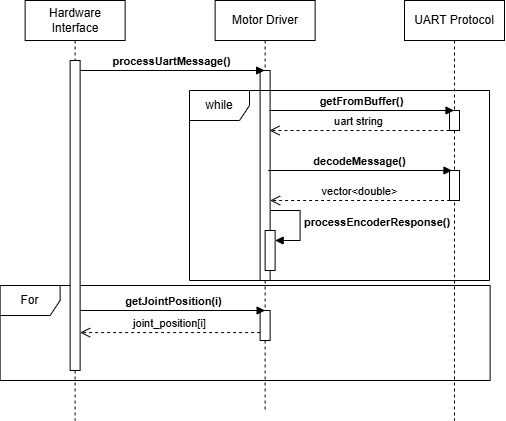
\includegraphics[width=0.8\linewidth]{Images/Implementation/Control/Read_flow.jpg}
    \caption{Luồng đọc (Read) của DensoInterface}
    \label{fig:placeholder}
\end{figure}

Trong luồng đọc của Arctos Interface, dữ liệu thực tế được phản hồi từ cánh tay cần được xử lý và đọc vào các state interfaces. Ở đầu hàm \lstinline[style=inlinecode]{read}, \lstinline[style=inlinecode]{processUartMessage()} của Motor Driver được gọi. Trong \lstinline[style=inlinecode]{processUartMessage}, hàm sẽ lần lượt lấy từng dữ liệu UART nhận được từ buffer của module UART và thực hiện decode (giải mã) nó theo format dữ liệu đã được đề xuất ở phần trước, sử dụng hàm decode được hỗ trợ từ module Uart. Sau khi decode, ta có được giá trị góc xoay của cả 6 trục trong một mảng số thực. Các giá trị góc xoay này sẽ lần lượt được lưu vào \lstinline[style=inlinecode]{JointConfig} của từng trục, sẵn sàng để được truy vấn.

Sau khi đã phân tích hết toàn bộ dữ liệu trong buffer UART, DensoInterface sẽ gọi \lstinline[style=inlinecode]{getJointPosition()} để lấy dữ liệu vị trí đã lưu bởi Motor Driver, cập nhật vào từng state interface tương ứng: \lstinline[style=inlinecode]{joint_position_[i]}.

% \begin{figure}[H]
%     \centering
%     \includegraphics[width=0.72\linewidth]{Images/Implementation/Control/DensoHand_Read_flow.jpg}
%     \caption{Luồng đọc (Read) của DensoHandInterface}
%     \label{fig:denso-hand-read-flow}
% \end{figure}

Chuyển qua luồng đọc của DensoHandInterface, ta cần trước nhất gọi \lstinline[style=inlinecode]{writeQueryCommand()} xuống tay gắp để hỏi trạng thái (vì trạng thái không được liên tục gửi lên như phía cánh tay). Sau khi nhận được phản hồi, hàm \lstinline[style=inlinecode]{processUartMessage()} của ServoDriver thực hiện công việc liên tục lấy chuỗi UART từ buffer đã lưu, và thực hiện decode, bóc tách dữ liệu JSON ngay trên Servo Driver. Giá trị "pos" từ câu trả lời của Driver-Hat-A được tính toán thêm một số bước để chuyển thành giá trị góc phù hợp, đơn vị rad, và gán vào state interface của DensoHandInterface.

\subsection{Ros2 Controllers}

Ros2 controllers là lớp thứ 3 trong kiến trúc Ros2 Control, đảm nhiệm vai trò tạo ra những bộ điều khiển (controller) làm nhiệm vụ cập nhật (update) trong chuỗi chu kì ba bước: read-update-write. Với việc dùng Ros2 Control, người dùng có thể tự mình viết một bộ controller riêng, hoặc tận dụng những controller đã được phát triển sẵn bởi framework. Những controller được phát triển này đã được tổng quát hóa để phù hợp cho nhiều loại robot thông dụng khác nhau, cũng như có khả năng tích hợp tốt với MoveIt2 và Nav2. Chính vì vậy, đề tài ưu tiên sử dụng ba loại controller thông dụng cho dự án cánh tay robot có kèm tay gắp, bao gồm: JointTrajectoryController, GripperActionController và JointStateBoardcaster. Mỗi loại controller được khởi tạo với một tên riêng biệt, nhằm phục vụ mục tiêu điều khiển khác nhau.

Trước nhất, ta cần cấu hình thuộc tính chung cho controller manager trong file ros2\_controller.yaml, cụ thể:

\begin{lstlisting}
controller_manager:
  ros__parameters:
    update_rate: 10 #Hz
    denso_arm_controller:
      type: joint_trajectory_controller/JointTrajectoryController

    denso_hand_controller:
      type: position_controllers/GripperActionController

    joint_state_broadcaster:
      type: joint_state_broadcaster/JointStateBroadcaster
\end{lstlisting}

Phần cấu hình này gồm 2 phần quan trọng: cấu hình update\_rate, là chu kì hoạt động của 1 chu trình read-update-write, và khai báo danh sách các tên controller kèm theo loại của chúng. Chu kì hoạt động hiện tại đang được chọn là 10Hz, nghĩa là mỗi chu kì read-update-write sẽ xảy ra mỗi 100ms. Mặc dù chu kì hoạt động khá thấp so với các dự án khác, tuy nhiên lại là một giá trị phù hợp và đem lại sự ổn định cho hệ thống hiện tại. Lý do của việc cập nhật và điều khiển mỗi 100ms là do:

\begin{itemize}
    \item Máy RC5 xử lý nhận string UART mỗi 10ms.
    \item Khi truyền lệnh điều khiển (write) từ RC5 xuống UART, lệnh sẽ phải được phân tích theo dạng chuỗi một cách thủ công, mất khoảng 20-30ms
    \item Khi xử lý lệnh xong, cánh tay robot cần mất một khoảng thời gian để xoay. Do giới hạn về mặt cơ học cánh tay, cánh tay có thể không thể đạt đến vị trí yêu cầu trong khoảng thời gian ngắn. 
\end{itemize}

Với 100ms, trừ đi thời gian nhận UART và xử lý lệnh điều khiển, cánh tay sẽ có tối thiểu 60ms để xoay tới vị trí được yêu cầu cho tới khi nhận lệnh tiếp theo, là một khoảng thời gian phù hợp, xem xét giới hạn về mặt cơ học hiện tại. Thử nghiệm cho thấy cánh tay sẽ quay tới vị trí yêu cầu trễ khoảng 1-2s cho một lần planning và execute với MoveIt2. Mặt khác, việc tăng tần số lên sẽ chỉ khiến số lượng lệnh gửi xuống tăng lên nhiều hơn, thời gian robot đươc phép xoay sẽ giảm, từ đó làm tăng cao thời gian trễ cho mỗi lần thực hiện chuỗi hành động xoay. 

Tiếp đến, cấu hình của từng controller, và cách nó liên kết với hardware interface sẽ được trình bày.

\subsubsection{denso\_arm\_controller}

"Denso\_arm\_controller" thuộc loại JointTrajectoryController, đóng vai trò chính trong việc vận hành hoạt động của cánh tay robot. Trang \href{https://control.ros.org/humble/doc/ros2_controllers/joint_trajectory_controller/doc/userdoc.html}{JointTrajectoryController} của Ros2-Control cung cấp chi tiết cách để cấu hình và sử dụng loại controller này, cũng như những chức năng mà controller hỗ trợ. Cấu hình cho phần Denso\_arm\_controller hiện tại bao gồm danh sách các trục sẽ điều khiển, state interface, command interface cùng một số thuộc tính đặc biệt:

\begin{lstlisting}
denso_arm_controller:
  ros__parameters:
    joints:
      - X_joint
      - Y_joint
      - Z_joint
      - A_joint
      - B_joint
      - C_joint
    command_interfaces:
      - position
    state_interfaces:
      - position

    state_publish_rate: 25.0
    action_monitor_rate: 10.0

    allow_partial_joints_goal: false
    state_tolerance_check: false  # Disable tolerance checking for simplicity

    allow_nonzero_velocity_at_trajectory_end: true
\end{lstlisting}

Cấu hình hiện tại cho biết Denso\_arm\_controller sẽ có 6 trục, mỗi trục đều có position interface cho command (lệnh điều khiển) và state (trạng thái). Khi chạy controller, trạng thái của controller được cung cấp ở dạng topic với tần số 25hz, và khi thực hiện action, việc theo dõi sự thay đổi trạng thái được thực hiện với tần số 10hz. Tuy nhiên, việc cấu hình ở file yaml là chưa đủ để có thể khởi chạy một luồng ros2-control gồm controller-interface hoàn chỉnh, mà nó cần có sự ràng buộc ở nhiều vị trí khác nhau để đảm bảo liên kết giữa các module được đồng nhất. Cụ thể, cấu hình "6 trục, mỗi trục đều có position interface cho command (lệnh điều khiển) và state (trạng thái)" cần tương đồng trong:

\begin{enumerate}
    \item \textbf{File Urdf}: Dưới tag <ros2\_control>, ngoài thông tin về plugin "hardware interface" sẽ sử dụng, cần liệt kê rõ các joint với tên trùng với tên joint đã cấu hình trong file yaml, đi kèm với command interface và position interface. Ví dụ của trục "X\_joint" dưới tag <ros2\_control> và các trục khác phải có cấu trúc:
    \begin{lstlisting}[language=xml]
    <joint name="X_joint">
        <command_interface name="position">
          <param name="min">-2.967060</param>
          <param name="max">2.967060</param>
        </command_interface>
        <state_interface name="position">
          <param name="initial_value">${initial_positions['X_joint']}</param>
        </state_interface>
    </joint>
    \end{lstlisting}
    \item \textbf{File hiện thực DensoInterface}: Ở bước export state/command interface, loại và số lượng interface cho từng trục cần được export đủ và chính xác, ví dụ:
    \begin{lstlisting}[language=C]
state_interfaces.emplace_back(
            info_.joints[i].name, hardware_interface::HW_IF_POSITION, &joint_position_[i]);
...
command_interfaces.emplace_back(
            info_.joints[i].name, hardware_interface::HW_IF_POSITION, &joint_position_command_[i]);
    \end{lstlisting}
    Hai câu lệnh trên đảm bảo joint với tên được ghi trong URDF dưới tag <ros2\_control> (ví dụ X\_joint) sẽ được cung cấp hai command interface và state interface loại Position bởi DensoInterface.
\end{enumerate}

Nếu có sự không đồng nhất giữa cấu hình file yaml, urdf hoặc cách hardware interface export, controller tương ứng sẽ không khởi chạy.

Khi cấu hình hoàn chỉnh và khởi chạy được denso\_arm\_controller, controller này sẽ cung cấp hai cách thức để điều khiển: 

\begin{itemize}
    \item Thông qua Action: denso\_arm\_controller/follow\_joint\_trajectory
    \item Thông qua Ros topic: denso\_arm\_controller/joint\_trajectory
\end{itemize}

Hai cách thức giao tiếp này sẽ được tận dụng bởi MoveIt2 trong chức năng planning và moveit servo. Chi tiết này sẽ được trình bày cụ thể hơn ở phần sau.

\subsubsection{denso\_hand\_controller}

"Denso\_hand\_controller" thuộc loại \textbf{GripperActionController}, là một loại controller đơn giản hơn với mục tiêu là điều khiển loại tay gắp hai đầu song song (parallel gripper). Tượng tự, cách cấu hình trong file ros2\_controlles.yaml có thể tham khảo ở trang \href{https://control.ros.org/humble/doc/ros2_controllers/gripper_controllers/doc/userdoc.html}{Gripper Action Controller}. Cấu hình hiện tại cho phần tay gắp là:

\begin{lstlisting}
denso_hand_controller:
  ros__parameters:
    joint: gripper_gear_right_joint

    goal_tolerance: 0.1               # rad
    stall_velocity_threshold: 0.001   # rad/s
    stall_timeout: 2.0                # seconds
    action_monitor_rate: 10.0         # Hz
\end{lstlisting}

So với JointTrajectoryController, GripperActionController chỉ điều khiển duy nhất một trục, và các tham số cấu hình cũng tương đối đơn giản. GripperActionController có yêu cầu cố định về interface, phải có hai state interface: velocity, position và một command interface: position. Về mặt điều khiển, chỉ cần cấu hình phần joint của tay gắp bên trái, phần joint còn lại sẽ bắt chước - mimic theo trong minh họa Rviz cũng như Gazebo. Các thông số liên quan tới tolerance, stall được chỉnh tương đối để tạo sự thoải mái trong điều khiển.

Tương tự, để có thể khởi chạy denso\_hand\_controller, ta cần đảm bảo những cấu hình ở các file liên quan được đồng nhất, cụ thể:

\begin{enumerate}
    \item Trong tag <ros2\_control> cho controller tay gắp, chỉ cần để một joint duy nhất, kèm theo một position interface và hai state interface. Tuy vậy, chỉ có position state interface sẽ được sử dụng trong dự án.
    \begin{lstlisting}[language=xml]
    <joint name="gripper_gear_right_joint">
        <command_interface name="position">
          <param name="min">0.087266</param>
          <param name="max">1.48353</param>
        </command_interface>
        <state_interface name="position">
          <param name="initial_value">${initial_positions['gripper_gear_right_joint']}</param>
        </state_interface>
        <state_interface name="velocity" />
    </joint>
    \end{lstlisting}
    \item Trong DensoHandInterface, các interfaces tương ứng cũng cần được export dầy đủ:
    \begin{lstlisting}
state_interfaces.emplace_back(
            info_.joints[i].name, hardware_interface::HW_IF_POSITION, &servo_position_[i]);
    ...
state_interfaces.emplace_back(
            info_.joints[i].name, hardware_interface::HW_IF_VELOCITY, &servo_velocity_[i]);
    ...
command_interfaces.emplace_back(
            info_.joints[i].name, hardware_interface::HW_IF_POSITION, &servo_position_command_[i]);
    \end{lstlisting}
\end{enumerate}

Denso\_hand\_controller cung cấp một phương thức giao tiếp duy nhất là thông qua \href{https://docs.ros.org/en/melodic/api/control_msgs/html/action/GripperCommand.html}{GripperCommand Action}, cụ thể: /denso\_arm\_controller/GripperCommand. Action server này được sử dụng bởi MoveIt2 cho planning, và cũng là cách điều khiển mà ứng dụng VR sử dụng để có thể nhanh chóng điều khiển tay gắp.

\subsubsection{joint\_state\_boardcaster}

Joint\_state\_boardcaster - như tên gọi - là một controller không phải để điều khiển thiết bị, mà là để thông báo (boardcast) dữ liệu. Đây cũng là một controller quan trọng, có nhiệm vụ thu thập toàn bộ state interface liên quan tới Joint và publish nó lên topic \textbf{/joint\_states}, cung cấp dữ liệu thực tế của phần cứng cho các ứng dụng quan tâm. Đối với controller này, đề tài để mọi thông số ở dạng mặc định và không tùy chỉnh gì thêm.

\subsection{Moveit2}

MoveIt2 là lớp thứ 4 trong kiến trúc đề xuất này, đóng vai trò là một giải pháp giúp điều khiển robot một cách hiệu quả với sự tích hợp chặt chẽ với Ros2-Control. Moveit2 sẽ tự động kết nối với Ros2-Control để điều khiển các Controller thực hiện chức năng "update". \href{https://moveit.picknik.ai/humble/doc/examples/setup_assistant/setup_assistant_tutorial.html}{MoveIt Setup Assistant} là một bộ tool được đề tài tận dụng để có thể sinh ra những file cấu hình cần thiết cho việc sử dụng MoveIt2, cũng như tạo sự liên kết giữa MoveIt2 và các Ros2-Controller đã chuẩn bị. Bộ tool hỗ trợ sinh ra thư mục "moveit\_config", gồm một số file chính như sau:

\begin{Verbatim}
moveit_config
└── config
    ├── arctos.srdf
    ├── initial_positions.yaml
    ├── joint_limits.yaml
    ├── chomp_planning.yaml
    ├── kinematics.yaml
    ├── moveit_controllers.yaml
    ├── moveit.rviz
    ├── pilz_cartesian_limits.yaml
    └── ros2_controllers.yaml
\end{Verbatim}

\begin{itemize}
    \item \textbf{arctos.srdf}: khác với file URDF có vai trò đặc tả về cấu trúc của robot, file SRDF (Semantic Robot Description Format) dùng để định nghĩa những thông tin ngữ nghĩa (semantic) cho robot. Ở đây có thể định nghĩa một nhóm các trục để điều khiển - planning trong \lstinline[style=inlinecode]{<group>}, định nghĩa trạng thái nhóm các trục và vị trí các trục ở trạng thái đó trong \lstinline[style=inlinecode]{<group_state>}. \lstinline[style=inlinecode]{<disable_collisions>} hữu dụng trong quá trình mô phỏng cánh tay robot, với khả năng tắt tính toán va chạm giữa những bộ phận của robot do nhiều lý do khác nhau, qua đó tăng tốc thời gian tính toán va chạm, cho phép MoveIt có thể lập ra những kế hoạch di chuyển (planning) chính xác, hiệu quả cho cánh tay robot.
    \item \textbf{chomp\_planning.yaml}: File cấu hình thuật toán tính toán lập quỹ đạo chuyển động Covariant Hamiltonian Optimization for Motion Planning (CHOMP). 
    \item \textbf{initial\_positions.yaml}: Vị trí ban đầu của từng trục cánh tay
    \item \textbf{joint\_limits.yaml}: Một file cấu hình khác cho phép ghi đè những thuộc tính trên file URDF của cánh tay, cụ thể là cấu hình về vận tốc và gia tốc tối đa. Việc cấu hình tốc độ/gia tốc tối đa có ảnh hưởng tương đối với MoveIt trong quá trình lập kế hoạch di chuyển của các trục, bởi MoveIt sẽ điều chỉnh vị trí và vận tốc linh hoạt, có tăng tốc ở khoảng bắt đầu và giảm tốc ở khoảng kết thúc, vận tốc trong quá trình di chuyển giữa sẽ gần đạt tối đa. Chính vì vậy, vận tốc tối đa càng cao, thời gian xoay cánh tay và số bước thực hiện hành động xoay càng ngắn. Ngược lại, vận tốc tối đa càng thấp, số bước di chuyển càng nhiều và cánh tay sẽ xoay chậm hơn.
    \item \textbf{kinematics.yaml}: File lựa chọn thuật toán động học sử dụng, thời gian tìm kiếm lời giải và timeout khi lời giải không thể tìm thấy.
    \item \textbf{ros2\_controllers.yaml}: Bộ tool khi đọc file urdf có chứa tag <ros2\_control>, sẽ cho phép người dùng cấu hình các controller ngay trong giao diện tool. Tại đây ta có thể định nghĩa tên controller và gán loại controller tương ứng, gán các joint sẽ sử dụng cho controller, và xác định các interface được sử dụng. 
    \item \textbf{moveit\_controllers.yaml} Sau khi cấu hình các controller, tool sẽ cho phép cấu hình phần "moveit controller \textbf{manager}". "Moveit\_simple\_controller\_manager" được sử dụng để quản lý các controller từ phía Ros2-Control, khai báo loại controller và các tên trục mà MoveIt sẽ điều khiển. Điều này giúp MoveIt2 biết rằng nó nên giao tiếp với Action Server của FollowJointTrajectory cho việc điều khiển cánh tay thông qua controller denso\_arm\_controller, và Action Server GripperCommand để điều khiển tay gắp thông qua denso\_hand\_controller.
\end{itemize}

Khi Cấu hình và khởi chạy thành công, MoveIt2 sẽ cho phép người dùng sử dụng tính năng "Planning" để tính toán quỹ đạo chuyển động tới một vị trí cụ thể (dựa vào tọa độ, hoặc giá trị các trục ở vị trí đích). Cơ chế planning này cũng sẽ hỗ trợ trong việc tính toán quỹ đạo chuyển động né vật cản được tạo trong môi trường Rviz, tùy theo yêu cầu của bài toán cần phát triển. Việc tính toán quỹ đạo chuyển động có thể được tùy chỉnh để dùng nhiều loại thuật toán khác nhau, và hiện tại đề tài đang dùng mặc định thuật toán CHOMP cho tính toán. Khi thấy planning đã ổn định, tính năng "Execute" yêu cầu MoveIt2 điều khiển các controller để xoay cánh tay robot theo quỹ đạo đã tính toán. Nhờ có sự trợ giúp của MoveIt2, các quỹ đạo đươc tính ra thường đã bao gồm tinh chỉnh, có sự tăng tốc ở giai đoạn đầu quỹ đạo và giảm tốc ở giai đoạn cuối, để giúp cho chuyển động trên quỹ đạo được mượt mà khi các lệnh điều khiển được gửi xuống khối controller.  

Ngoài khối planning, MoveIt2 cũng hỗ trợ package \href{https://moveit.picknik.ai/main/doc/examples/realtime_servo/realtime_servo_tutorial.html}{"MoveIt Servo"}, hay còn gọi là "Real-time Servo", cho nhu cầu điều khiển một hoặc nhiều trục xoay liên tục một góc nhỏ, hoặc điều khiển cánh tay di chuyển theo tọa độ X,Y,Z. Chi tiết tính năng này sẽ được trình bày ở khối sau.

\subsection{Khối ứng dụng}

Khối ứng dụng bao gồm các khối các module nhỏ riêng biệt, được phát triển dựa trên sự hỗ trợ của MoveIt2 cho để điều khiển cánh tay robot thực tế. Ở lớp này, nhiều loại ứng dụng có thể được phát triển, tuy nhiên trong giới hạn đề tài hiện tại sẽ chỉ xây dựng lớp ứng dụng để cung cấp phương thức điều khiển cho thành phần bên ngoài muốn giao tiếp với hệ thống. Hiện tại, khối ứng dụng cho phép thiết bị bên ngoài (Kính VR) giao tiếp với Ros2 bên trong thông qua Denso Moveit Servo (Service Provider) và Denso Remote Control (Action Server).

\subsubsection{Denso MoveIt Servo}

Denso MoveIt Servo là một Ros2 Service Provider, đóng vai trò như một Wrapper trên Ros2-Moveit-Servo để cung cấp khả năng điều khiển robot xoay từng trục hoặc theo tọa độ. Moveit-Servo cho phép người dùng thực hiện cấu hình cách hoạt động của module này qua file yaml, trong đó một số bộ cấu hình quan trọng có thể kể đến như:

\begin{lstlisting}
## Properties of outgoing commands
publish_period: 0.3  # 1/Nominal publish rate [seconds] 

# What type of topic does your robot driver expect?
command_out_type: trajectory_msgs/JointTrajectory

# What to publish?
publish_joint_positions: true
publish_joint_velocities: false
publish_joint_accelerations: false

## Plugins for smoothing outgoing commands
smoothing_filter_plugin_name: "online_signal_smoothing::ButterworthFilterPlugin"
\end{lstlisting}

Publish period là thời gian giữa các lệnh gửi điều khiển từ MoveIt-Servo. Với MoveIt-Servo, sẽ có hai luồng điều khiển: từ người dùng gửi lệnh tới MoveIt-Servo, và từ MoveIt-Servo sẽ tiến hành tính toán, đưa ra lệnh phù hợp để gửi thẳng tới Ros2-controller được cấu hình, thông qua topic thuộc loại "command\_out\_type". Với Publish period là 0.3, có nghĩa là cứ 300ms, MoveIt-Servo sẽ gửi một chuỗi quỹ đạo (JointTrajectory) tới Ros2-controller loại FollowJointTrajectory để yêu cầu xoay cánh tay, thay vì thông qua Action Server mà MoveIt2 sử dụng cho module planning thông thường. Điều này giúp MoveIt-servo có thể điều khiển thiết bị nhanh mà không bị ảnh hưởng bởi thời gian xử lý tương đối chậm của Action Server. Thêm nữa, ButterworthFilterPlugin được sử dụng để "lọc" dữ liệu điều khiển truyền ra, giúp các lệnh điều khiển ổn định và đảm bảo robot có thể xoay đều, mượt mà. 

\begin{lstlisting}
## Stopping behaviour
# Stop servoing if X seconds elapse without a new command
incoming_command_timeout:  0.3  
\end{lstlisting}

Một trong những vấn đề khi hiện thực việc điều khiển robot xoay liên tục, đó là xác định khi nào nên dừng việc xoay. MoveIt-Servo giải quyết điều này dễ dàng qua việc cho phép người dùng điều chỉnh thông số timeout, trong trường hợp này là 300ms; nghĩa là người dùng có thể spam liên tục lệnh điều khiển gửi tới MoveIt-Servo, tuy nhiên nếu ngưng gửi lệnh và MoveIt-Servo nhận thấy đã quá 300ms kể từ khi nhận lệnh cuối cùng, MoveIt-Servo cũng sẽ ngưng gửi lệnh JointTrajectory xuống controller, từ đó ngưng xoay robot thực tế. 

Tuy nhiên, cơ chế này lại mang tính ràng buộc về thời gian thực (Real-time) để có thể hoạt động chính xác. Cụ thể, cách MoveIt-Servo xác định timeout là lấy thời điểm trong Header TimeStamp có trong mỗi lệnh gửi tới MoveIt-Servo, trừ với thời gian thực tế (Ros wall-timer), điều này yêu cầu lệnh gửi tới phải có TimeStamp hợp lệ để MoveIt-Servo có thể tính toán và cho dừng hoạt động điều khiển sau khoảng thời gian timeout. 

\begin{lstlisting}
## Topic names
cartesian_command_in_topic: ~/delta_twist_cmds  
joint_command_in_topic: ~/delta_joint_cmds
joint_topic: /joint_states
status_topic: ~/status 
command_out_topic: /denso_arm_controller/joint_trajectory 
\end{lstlisting}

Phần cấu hình này giúp định nghĩa tên của các topic gửi tới MoveIt-Servo (in\_topic) và topic được gửi ra từ MoveIt-Servo tới Ros2-Controller (out\_topic). Như đã trình bày ở trên, MoveIt-Servo cho phép di chuyển cánh tay theo trục (joint\_command) hoặc theo tọa độ cartesian (cartesian\_command), tuy nhiên đề tài chủ yếu sử dụng joint\_command. Việc di chuyển theo tọa độ đề các còn một số điểm bất ổn định và cần nhiều kiểm tra kĩ hơn trước khi sử dụng chính thức. 

joint\_topic được cung cấp để giúp MoveIt-Servo tính toán quỹ đạo từ vị trí hiện tại của cánh tay. Chính vì vậy, trong trường hợp cánh tay thực tế quay trễ hơn so với lệnh điều khiển, cơ chế này sẽ khiến cánh tay bị "giật lùi". Giả sử, trục X được MoveIt-Servo tính toán, và gửi quỹ đạo quay lần lượt là [3, 5, 10, 15], mong đợi rằng cánh tay sẽ xoay tới vị trí 15 độ sau 300ms. Tuy nhiên, 300ms sau, cánh tay thực tế chỉ mới quay tới 7 độ (trạng thái của joint\_states), nên MoveIt-Servo tính lại quỹ đạo: [7, 10, 15, 18]. Tuy nhiên, lệnh 10, 15 đã được gửi tới Ros2-Control, và Ros2-Control đã truyền chúng xuống RC5 để thực thi, dẫn tới RC5 sẽ nhận chuỗi lệnh là: [3, 5, 10, 15, \textbf{7, 10, 15}, 18]. Trục X sẽ bị điều khiển xoay tới 15 độ rồi giật ngược về 7 độ, xoay tiếp lên 10, 15 trở lại.

Để tạm thời giải quyết vấn đề từ MoveIt-Servo có mong đợi không chính xác về thời gian xoay của cánh tay, cũng như độ trễ do tính chất cơ khí của cánh tay robot, đề tài hiện thực cơ chế Trend Learning ở lớp DensoInterface như đã trình bày ở phần trước, nhằm mục tiêu phát hiện chuỗi lệnh có xu hướng tăng/giảm, nên khi nhận lệnh giật lùi trong một khung thời gian nhỏ từ MoveIt-Servo tới denso\_arm\_controller, xuống DensoInterface, các lệnh giật lùi sẽ bị loại bỏ và thay bằng một giá trị hợp lệ trước đó + padding nhỏ. Điều này giúp giải quyết:

\begin{itemize}
    \item Loại bỏ tình huống giật lùi do cánh tay xoay chậm hơn so với mong đợi từ MoveIt-Servo
    \item Các lệnh giật lùi bị thay thế bằng giá trị hợp lệ cuối + padding thay vì ngưng gửi giúp cho RC5 luôn luôn có lệnh điều khiển ở mỗi chu kì của Ros2-control (100ms). Điều này giúp buffer RC5 sẽ luôn có lệnh và đảm bảo trục được xoay liên tục, tránh trường hợp xuất hiện khoảng trống lệnh, khiến trục xoay bị giật (giảm tốc và dừng vì đạt tới vị trí yêu cầu và không có lệnh mới (khoảng trống), sau đó lệnh hợp lệ mới được đưa vào, trục phải khởi động và tăng tốc để xoay)
\end{itemize}

Ngoài ra, MoveIt-Servo cũng đảm bảo rằng việc xoay từng trục được giới hạn bởi các limit được cấu hình từ file Urdf, khi gần chạm tới ngưỡng xoay của trục thì lệnh yêu cầu xoay sẽ bị chặn lại, không gửi tới Ros2-Controller, đảm bảo cho cánh tay hoạt động trong ngưỡng an toàn. 

Denso MoveIt Servo, như đã trình bày, sẽ có vai trò khởi tạo Node MoveIt-Servo với những cấu hình từ file yaml đã mô tả, từ đó cung cấp cho người sử dụng hai topic để điều khiển:

\begin{itemize}
    \item denso\_moveit\_servo\_node/delta\_twist\_cmds [geometry\_msgs::msg::TwistStamped]
    \item denso\_moveit\_servo\_node/delta\_joint\_cmds [control\_msgs::msg::JointJog] (*)
\end{itemize}

Kèm theo đó, hai dịch vụ (service) được cung cấp để cho phép sử dụng/ tắt MoveIt-Servo:

\begin{itemize}
    \item denso\_moveit\_servo\_node/start\_servo [std\_srvs::srv::Trigger]
    \item denso\_moveit\_servo\_node/stop\_servo [std\_srvs::srv::Trigger]
\end{itemize}

Chỉ khi dịch vụ ~/start\_servo được gọi, thì các lệnh gửi đến 2 topic delta\_twist\_cmds / delta\_joint\_cmds mới được xử lý bởi MoveIt-Servo. Ngược lại, nếu ~/stop\_servo được gọi, thì MoveIt-Servo sẽ không hoạt động, cho tới khi ~/start\_servo được trigger.

\subsubsection{Denso Remote Control}

Denso Remote Control được thiết kế ở dạng một Action Server, với mục tiêu cung cấp cho thiết bị bên ngoài phương thức để gửi lệnh điều khiển cánh tay tới một vị trí cụ thể (thông qua giá trị của 6 trục hoặc tọa độ XYZ) xuống MoveIt để planning và thực thi. Lý do lựa chọn Action Server thay vì Service Provider là vì thao tác Planning, đặc biệt là Execute của MoveIt có thời gian thực hiện dài, nên dùng Action Server sẽ giúp cho thiết bị bên ngoài có thể gửi mục tiêu (Goal) và theo dõi trạng thái thực thi cho tới khi hoàn thành. 

Denso Remote Control sử dụng một định dạng Action riêng, gọi là \textbf{MoveToPose}, bao gồm ba message:

\begin{lstlisting}[language={}]
# Request
geometry_msgs/Pose pose
float64[] joints
bool use_pose
---
#Result
bool completed
---
#Feedback
string step
\end{lstlisting}

Trong đó, Request sẽ chấp nhận message dạng geometry\_msgs/Pose (mô tả tọa độ XYZ và góc xoay của phần đầu cánh tay - end effector) hoặc giá trị góc (độ) của sáu trục cánh tay robot. Biến bool use\_pose dùng để quyết định message pose sẽ được sử dụng (true) hay chuỗi sáu góc của cánh tay robot sẽ được sử dụng (false). Result là \lstinline[style=inlinecode]{bool completed}, cho biết Action server đã hoàn thành công việc chưa, và \lstinline[style=inlinecode]{string step} cập nhật trạng thái của từng bước hoạt động của action server, trong quá trình nhận lệnh, planning và execute từ phía MoveIt.

Luồng hoạt động và phản hồi của Denso Remote Control khi có request từ Action client sẽ theo như hình:

\begin{figure}[H]
    \centering
    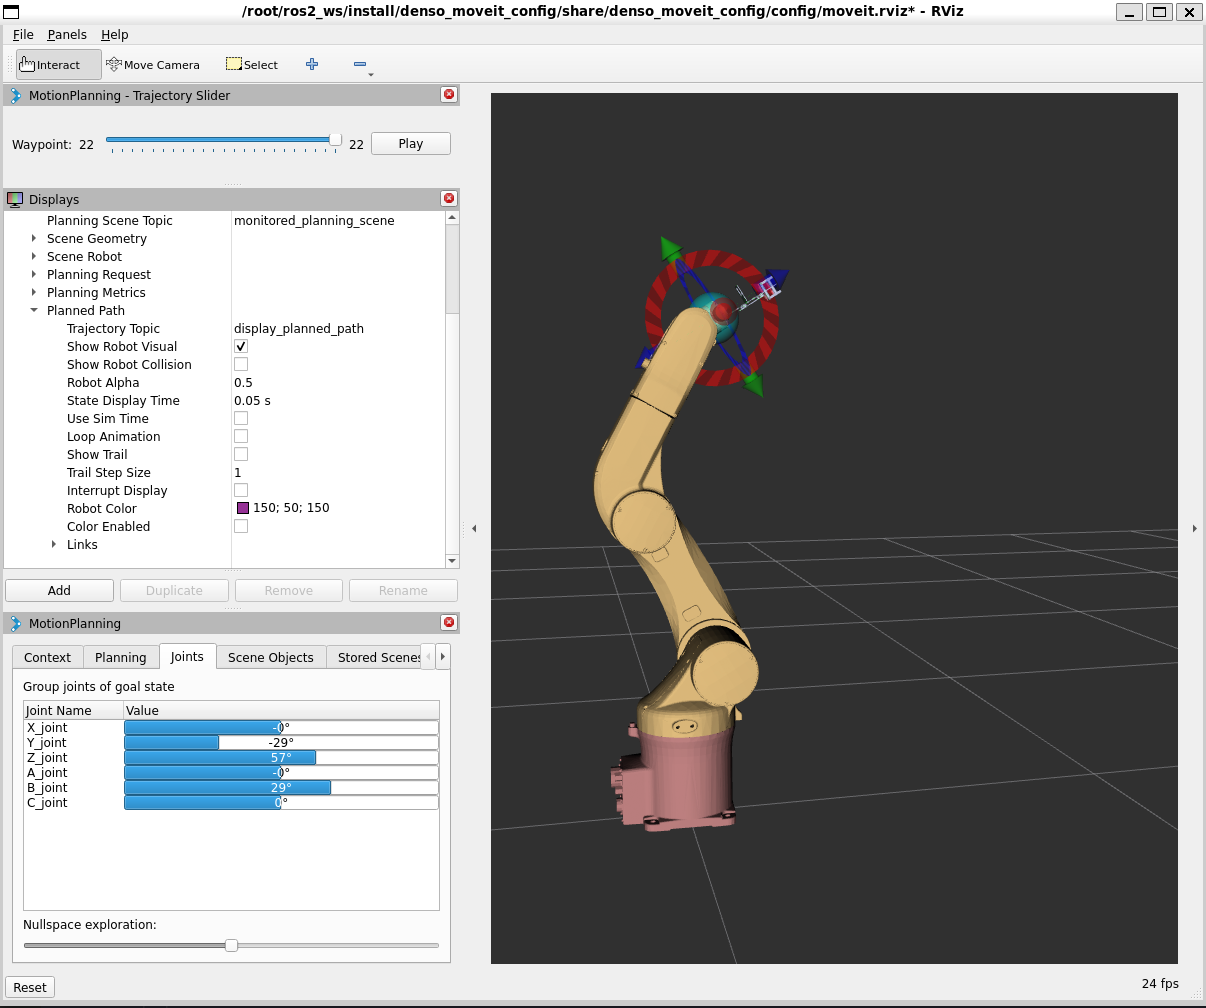
\includegraphics[width=0.75\linewidth]{Images/Implementation/remote_control_1.png}
    \caption{Luồng hoạt động của Denso Remote Control Action Server}
    \label{fig:denso-remote-control-flow}
\end{figure}

\begin{enumerate}
    \item Khi nhận một Goal request, kiểm tra \lstinline[style=inlinecode]{use\_pose} và quyết định chọn message Pose hay chuỗi góc trục. Nếu request đưa tới là hợp lệ, tiến tới bước planning.
    \item Thực hiện ghi trạng thái đích (sử dụng \lstinline[style=inlinecode]{setPoseTarget()} nếu dùng pose, hoặc \lstinline[style=inlinecode]{setJointValueTarget()} nếu dùng chuỗi góc trục), sau đó tiến hành planning thông qua Moveit. \lstinline[style=inlinecode]{step} hiển thị "planning". Nếu planning thất bại, \lstinline[style=inlinecode]{completed = true} và \lstinline[style=inlinecode]{step = planning_failed:} kèm theo lý do cụ thể.
    \item Sau khi planning thành công, bước execute sẽ khởi chạy sử dụng hàm \lstinline[style=inlinecode]{execute()} của MoveIt, \lstinline[style=inlinecode]{step = executing} và thiết bị sẽ được điều khiển trong suốt thời gian executing. Nếu có lỗi trong quá trình execute, \lstinline[style=inlinecode]{step = execute_failed:} kèm lý do, và \lstinline[style=inlinecode]{completed = true}. Nếu việc execute thành công, \lstinline[style=inlinecode]{step = completed} và \lstinline[style=inlinecode]{completed=true}
\end{enumerate}

Khi khởi chạy, Action client có thể gửi MoveToPose goal request tới Denso Remote Control để thực hiện việc xoay cánh tay robot tới vị trí yêu cầu.

\paragraph{Đánh giá nhanh thiết kế điều khiển}

Thiết kế hiện tại cho thấy sự cân bằng giữa độ ổn định và khả năng mở rộng: các lớp Driver, Hardware Interface, Controller và lớp ứng dụng đã được tách rõ để dễ kiểm thử và bảo trì. Cơ chế CRC theo độ dài payload ở phía RC5 cùng Ring Buffer giúp tăng khả năng chịu lỗi khi truyền UART. Tuy vậy, một số giới hạn vẫn còn tồn tại, điển hình là độ trễ cơ khí khiến MoveIt Servo đôi khi tạo chuỗi lệnh có xu hướng giật lùi; giải pháp Trend Learning ở DensoInterface hiện đang xử lý tốt ở mức ứng dụng, nhưng vẫn cần thêm các thử nghiệm định lượng dài hạn để đánh giá độ bền vững theo nhiều kịch bản tải khác nhau.

\subsection{Mô phỏng với Gazebo}

Trong quá trình phát triển, để giảm bớt sự phụ thuộc vào thiết bị thực tế và tăng tốc thời gian phát triển các module lớp ứng dụng trở lên, Gazebo Ignition được xây dựng để làm hệ thống mô phỏng điều khiển thay thế phần Hardware Interface trở xuống. Việc tận dụng Gazebo trong quá trình phát triển ứng dụng giúp nhà phát triển có thể nhanh chóng kiểm tra cách hoạt động của robot trong chuỗi điều khiển của mình, và thực hiện sửa đổi cho phù hợp, giảm gánh nặng và khả năng lỗi lên thiết bị thực tế. 

Để có thể tích hợp Gazebo vào dự án, ta sẽ cần thực hiện một số thay đổi sau:

\begin{enumerate}
    \item \textbf{Tắt trọng lực, bật động học}: Với mỗi một Link trong file UART, tag gazebo cần được liên kết để tắt tác dụng của trọng lực lên cánh tay. Bật động học đảm bảo cánh tay robot chỉ có thể được điều khiển bởi người dùng, chứ không chịu ảnh hưởng bởi va chạm với vật thể nào khác trong mô phỏng. Điều này giúp cho robot có thể giữ vị trí cố định và điều khiển được.

    \begin{lstlisting}[language=xml]
     <link name="${name}">
     ...
     </link>
    <gazebo reference="${name}">
      <kinematic>true</kinematic>
      <gravity>false</gravity>
    </gazebo>
    \end{lstlisting}
    
    \item \textbf{Thêm thuộc tính friction (ma sát), damping (giảm chấn) vào cho các trục trong file URDF}: Nếu thiếu hai thông số friction và damping, các trục gần như sẽ bị overshoot khi xoay do quán tính, khiến nó xoay xa hơn so với vị trí yêu cầu. Bộ số friction, damping hợp lý sẽ giữ cho cánh tay có được độ ổn định, có thể giữ vị trí góc được điều khiển và xoay với tốc độ gần tương đồng với thiết bị thật. 

        \begin{lstlisting}[language=xml]
    <joint name="${name}" type="${type}">
      ...
      <dynamics damping="${damping}" friction="${friction}"/>
    </joint>
    \end{lstlisting}
    \item \textbf{Tích hợp GazeboSimRos2ControlPlugin vào file URDF}: Gazebo cung cấp khả năng tích hợp dễ dàng với Ros2-Control, người dùng chỉ cần thêm Gazebo như một plugin như sau:

        \begin{lstlisting}[language=xml]
    <gazebo>
      <plugin filename="gz_ros2_control-system" name="gz_ros2_control::GazeboSimROS2ControlPlugin">
        <robot_param>robot_description</robot_param>
        <robot_param_node>robot_state_publisher</robot_param_node>
        <parameters>$(find denso_moveit_config)/config/ros2_controllers.yaml</parameters>
        <controller_manager_name>controller_manager</controller_manager_name>
      </plugin>
    </gazebo>
    \end{lstlisting}

    \item \textbf{Tạo file hook thay đường dẫn mặc định của Gazebo sang Ros2}: Do Gazebo là một phần mềm riêng biệt so với ROS2, nên khi khởi chạy, Gazebo sẽ không biết đường dẫn trỏ tới các tài nguyên như file mô hình 3D (STL) của cánh tay robot. Việc tạo file hooks ở ngay trong robot description sẽ giúp giải quyết vấn đề này.
    
    \item \textbf{Thay thế Hardware Interface với Gazebo}: Gazebo đóng vai trò là một bộ mô phỏng thiết bị vật lý, do đó nó cần đóng vai trò là một Hardware Interface để cung cấp trạng thái, cũng như thực hiện yêu cầu điều khiển. Khi cần sử dụng Gazebo, ta bật \lstinline[style=inlinecode]{sim=True}, và GazeboSimSystem sẽ thay thế HardwareInterface thực tế.

    \begin{lstlisting}[language=xml]
    <hardware>
        <!-- By default, set up controllers for gazebo. This won't work on real hardware -->
        <xacro:if value="${sim}">
          <plugin>gz_ros2_control/GazeboSimSystem</plugin>
        </xacro:if>
        <xacro:unless value="${sim}">
          <plugin>denso_interface/DensoInterface</plugin>
          <param name="device">/dev/ttyUSB0</param>
          <param name="baud_rate">115200</param>
          <param name="timeout">1000</param>
        </xacro:unless>
    </hardware>
    \end{lstlisting}

    \item Sau cùng, ở file launch của dự án, lần lượt khởi chạy Gazebo, sinh mô hình robot bằng cách dọc robot description, Gazebo sẽ xuất hiện và đóng vai trò là bộ mô phỏng cánh tay robot, có thể điều khiển được thông qua MoveIt và Ros2-Control.

\end{enumerate}

\subsection{Lấy dữ liệu camera với V4L2 Camera Node}

Để có thể điều khiển cánh tay robot hiệu quả trong môi trường ảo, việc theo dõi các hình ảnh camera từ hệ thống xung quanh thiết bị thực tế là cần thiết để theo dõi và tăng nhận thức môi trường cho người sử dụng. Chính vì vậy, đề tài chủ trương sử dụng hai camera: camera 1 ở đầu tay gắp và camera 2 bao quát môi trường và cánh tay. Cả hai camera đều là Usb Camera của Ugreen, kết nối trực tiếp tới máy PC Controller.

Để đọc được dữ liệu ảnh từ camera vào Ros2, đề tài sử dụng package \href{https://github.com/tier4/ros2_v4l2_camera}{ros2\_v4l2\_camera} đóng vai trò như ros node truyền dữ liệu camera theo những thông số cấu hình linh động ra các topic thông dụng về dữ liệu ảnh. Ảnh được truyền qua topic với kích thước [640 x 480], định dạng màu rgb8.

Thêm nữa, package \href{https://github.com/ros-perception/image_transport_plugins}{image\_transport\_plugins} được sử dụng để cung cấp khả năng nén ảnh, giúp người dùng có thể truyền dữ liệu ảnh đi với lượng data ít hơn, giảm bớt tải cho đường truyền. Chỉ cần cài đặt image\_transport\_plugins, ros2\_v4l2\_camera sẽ phát hiện plugin này và tự động tạo thêm topic \lstinline[style=inlinecode]{/image_raw/compressed} để truyền dữ liệu đã được nén bởi plugin.

Lệnh cài đặt ros2\_v4l2\_camera và image\_transport\_plugins như sau:

\begin{lstlisting}[style=bashstyle]
    sudo apt install ros-humble-v4l2-camera ros-humble-rqt-image-view ros-humble-image-transport-plugins -y
\end{lstlisting}

Trong đó \lstinline[style=inlinecode]{rqt-image-view} là một package dùng để kiểm tra nhanh chóng dữ liệu hình ảnh được truyền qua topic Camera trong môi trường Ros2.
 
Khi cài đặt và khởi chạy thành công, dữ liệu ảnh từ hai camera sẽ được truyền qua các topic sau đây, cho cả ảnh gốc (image\_raw) và ảnh đã nén (compressed)

\begin{lstlisting}[language={}]
    /camera_1/image_raw
    /camera_1/image_raw/compressed
    /camera_2/image_raw
    /camera_2/image_raw/compressed
\end{lstlisting}
 
\subsection{Sử dụng RosBridge server}

Ros2 cho phép giao tiếp dễ dàng thông qua mạng LAN cho các thiết bị cùng chạy Ros, tuy nhiên đối với kính VR chạy ứng dụng Unity, việc cài đặt và chạy Ros2 là không khả thi. \href{https://github.com/siemens/ros-sharp}{Ros-Sharp} cung cấp giải pháp giao tiếp giữa ứng dụng .Net (C\#, Unity) và Ros2 thông qua Web socket một cách hiệu quả và nhanh chóng.

\begin{figure}[H]
    \centering
    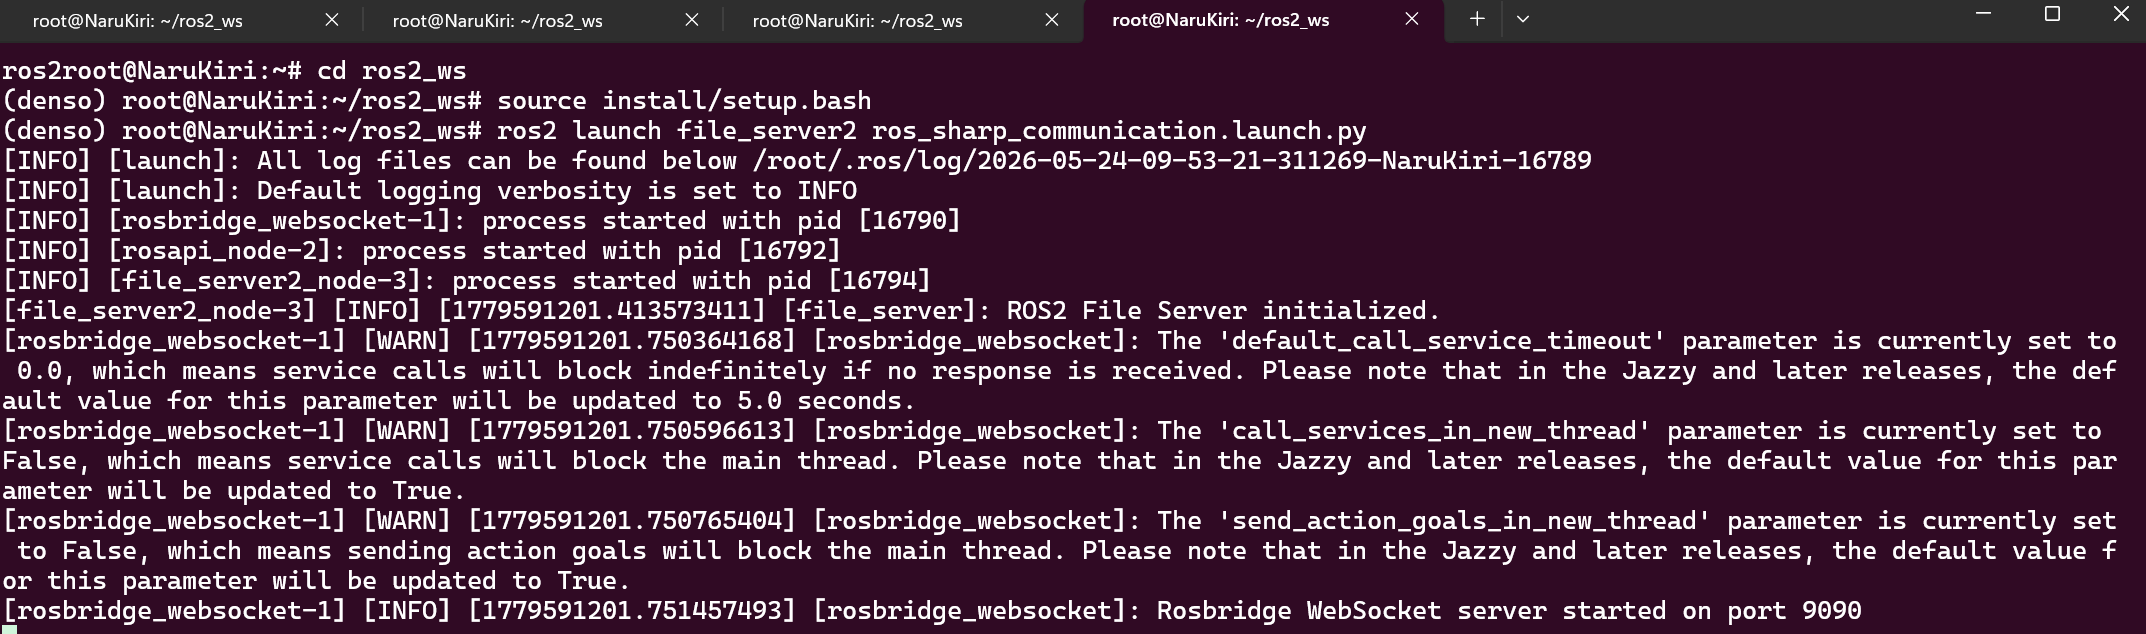
\includegraphics[width=0.8\linewidth]{Images/Implementation/rosbridge_server.png}
    \caption{RosBridge Server làm cầu nối giữa ROS2 và ứng dụng Unity}
    \label{fig:rosbridge-server}
\end{figure}

Để tạo kết nối cho giao tiếp Ros, người dùng cần cài đặt các package hỗ trợ ở cả phía Ros2 và cả Unity. Về phía Ros2, ta sẽ cài đặt RosBridge Server để cho phép ứng dụng Unity có thể kết nối tới. 

\begin{lstlisting}[style=bashstyle]
# Install rosbridge_suite
sudo apt-get install ros-humble-rosbridge-server
\end{lstlisting}

Sau khi cài xong, package \href{https://github.com/siemens/ros-sharp/tree/master/ROS%20Packages/ROS2/file_server2}{file\_server2} từ Repo được sử dụng để khởi chạy RosBridge server cùng một số tham số tùy chỉnh như port, kích thước gói tin, timeout cho service...

Với việc cài đặt RosBridge server, gần như mọi topic, service và action có thể được truy cập bởi ứng dụng .Net sử dụng Ros-sharp. Với đồ án hiện tại, RosBridge Server sẽ cho phép ứng dụng VR truy cập các topic và dịch vụ sau:

\begin{figure}[H]
    \centering
    \begin{subfigure}{0.48\linewidth}
        \centering
        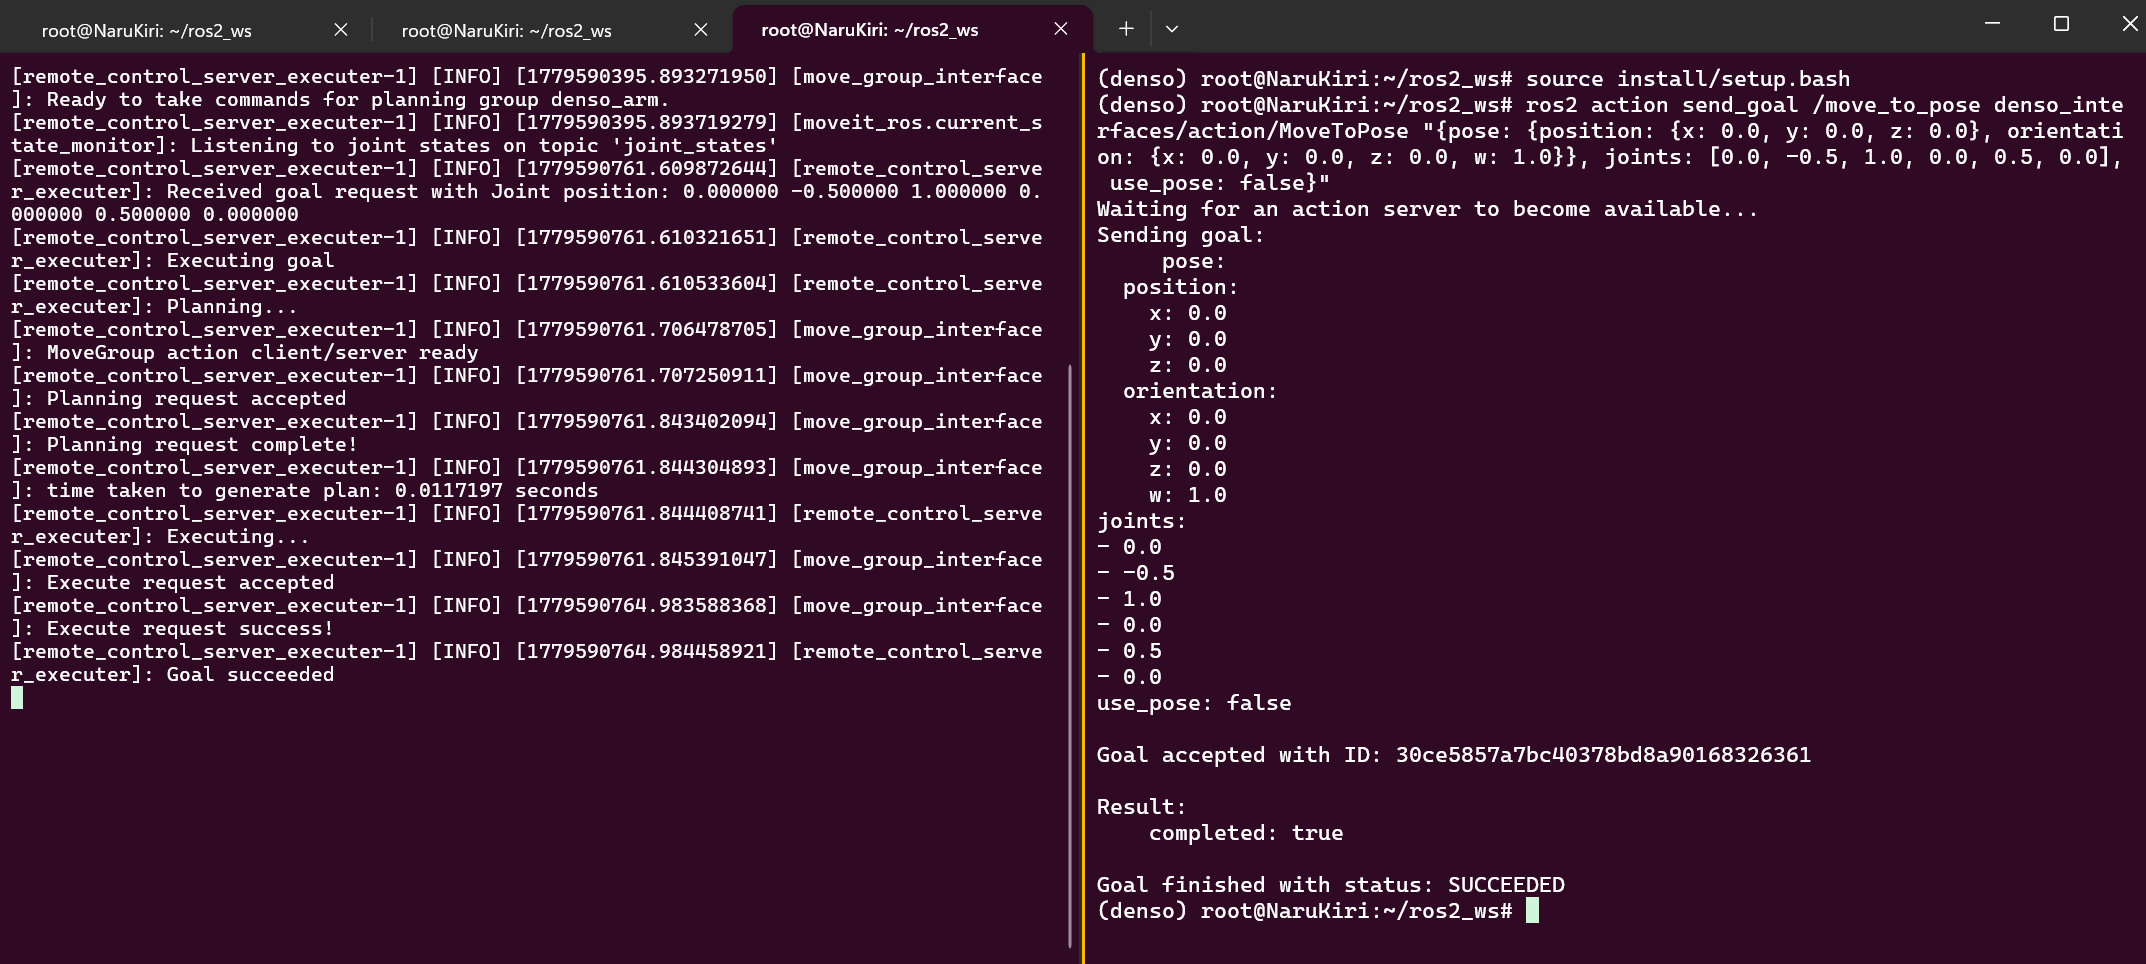
\includegraphics[width=\linewidth]{Images/Implementation/remote_control.png}
        \caption{Denso Remote Control}
    \end{subfigure}
    \hfill
    
    \caption{Các dịch vụ ROS2 chính mà ứng dụng VR truy cập qua RosBridge}
    \label{fig:rosbridge-services}
\end{figure}

Trong đó, \lstinline[style=inlinecode]{/joint_states} từ JointStateBoardcaster dùng để theo dõi trạng thái của cánh tay robot, Denso Remote Control Action Server để điều khiển cánh tay xoay tới vị trí xác định, Denso MoveIt Servo để xoay từng trục của cánh tay liên tục, và hai topic camera từ V4L2 node, để gửi hình ảnh từ camera gửi lên ứng dụng VR.

\section{Ứng dụng VR}

Ở phần này, phần thiết kế và xây dựng ứng dụng VR - module quan trọng thứ 3 của toàn bộ hệ thống, hoàn tất luồng điều khiển từ VR - Ros2 - RC5 của đề tài. Đối với việc xây dựng ứng dụng, đề tài chủ trương sử dụng phiên bản Unity mới nhất - Unity 6, để có thể tận dụng sức mạnh và các tính năng nổi bật từ Game Engine này, cũng như dễ dàng tích hợp với \href{https://developers.meta.com/horizon/downloads/package/meta-xr-sdk-all-in-one-upm/}{Meta XR SDK} để xây dựng ứng dụng VR. Mục tiêu mà ứng dụng VR cần đáp ứng là:
\begin{itemize}
    \item Dễ sử dụng, thân thiện với người dùng.
    \item Hiệu năng ổn định, không crash, FPS không dưới 60.
    \item Tính tương tác cao, đa dạng phương thức điều khiển 
\end{itemize}

\subsection{Chuẩn bị tài nguyên để xây dựng ứng dụng}

Để xây dựng \textbf{ứng dụng VR} điều khiển Robot với\textbf{ Ros2} trên Unity, trước nhất ta phải tiến hành cài đặt hai package quan trọng của ứng dụng, là \href{https://developers.meta.com/horizon/downloads/package/meta-xr-sdk-all-in-one-upm/}{Meta XR SDK} và \href{https://github.com/siemens/ros-sharp}{Ros-Sharp}.

\textbf{Meta XR SDK}

Meta XR SDK là một package lớn và tương đối phức tạp, nên Package này nên được ưu tiên cài đặt trước trên một dự án Unity mới. Chi tiết về cách thức cài đặt trên Unity, từ Import các assets liên quan, thay đổi cấu hình Project, bật hỗ trợ development mode của kính VR... đều được liệt kê rõ, từng bước tại trang \href{https://developers.meta.com/horizon/documentation/unity/unity-tutorial-hello-vr/}{Unity Hello World for Meta Quest VR headsets}

\textbf{Ros-Sharp và Import Robot vào ứng dụng}

Tiếp đến là cài đặt Ros-Sharp package trên Unity, qua đó cho phép giao tiếp với RosBridge Server đã cài đặt trên Ros2 trước đó. Việc cài đặt Ros-sharp cũng tương đối đơn giản, và mặc định package này cũng cung cấp các thao tác cơ bản nhất như kết nối tới Ros2, subscribe/publish vào một vài topic thông dụng của Ros2 cùng một bộ các kiểu dữ liệu Ros2 thông dụng. Điểm ấn tượng của gói package này là cho phép người dùng tự do định nghĩa message/service/action, và cho phép sinh ra các file class phù hợp trong C\# cho các message/service/action này thông qua việc import từ Ros. Tuy nhiên, việc import chỉ hỗ trợ cho việc định nghĩa format message/service/action, còn các hành động như publish, subscribe, gọi Service, gọi Action server và lấy kết quả/feedback... đều cần xây dựng thêm các class cho mỗi hành động, bởi tùy theo cấu trúc của messsage, mà hành động xử lý sẽ khác nhau.

Sau khi cài đặt thành công, người dùng có thể chuyển (transfer) mô hình 3D của robot vào trong Unity thông qua Ros-Sharp. Cách chính xác nhất để "tranfer" là mở một kết nối tới Ros2 đang chạy và đang publish Robot Description, sau đó thực hiện theo hướng dẫn \href{https://github.com/siemens/ros-sharp/wiki/User_App_ROS_TransferURDFFromROS}{TransferURDFFromROS} để đưa Robot vào trong môi trường Unity. Cách làm này đảm bảo mô hình 3D của robot được chuyển qua đầy đủ, kèm toàn bộ những script hỗ trợ đính kèm từng component cho việc đọc dữ liệu \lstinline[style=inlinecode]{\joint_states} để đồng bộ với robot thực tế.

Về phía Ros2, lần lượt chạy các lệnh sau ở hai cửa sổ terminal khác nhau để đảm bảo Robot Description được publish và RosBridge server được khởi động, sẵn sàng để nhận kết nối:

\begin{lstlisting}[style=bashstyle]
    ros2 launch denso_bringup denso_bringup.launch.py
    ros2 launch file_server ros_sharp_communication.launch.py
\end{lstlisting}

Sau đó, ở Unity, ta có thể chỉnh các đường dẫn và tên như sau để import mô hình 3D của robot từ ROS vào Unity

\begin{figure}[H]
    \centering
    \begin{subfigure}{0.48\linewidth}
        \centering
        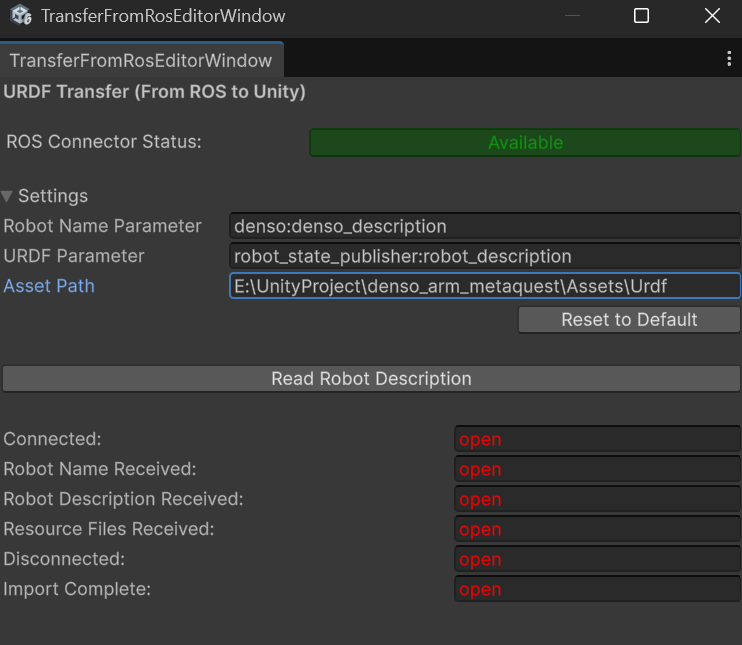
\includegraphics[width=\linewidth]{Images/Implementation/transferfromros.png}
        \caption{Thiết lập Transfer URDF from ROS}
    \end{subfigure}
    \hfill
    \begin{subfigure}{0.48\linewidth}
        \centering
        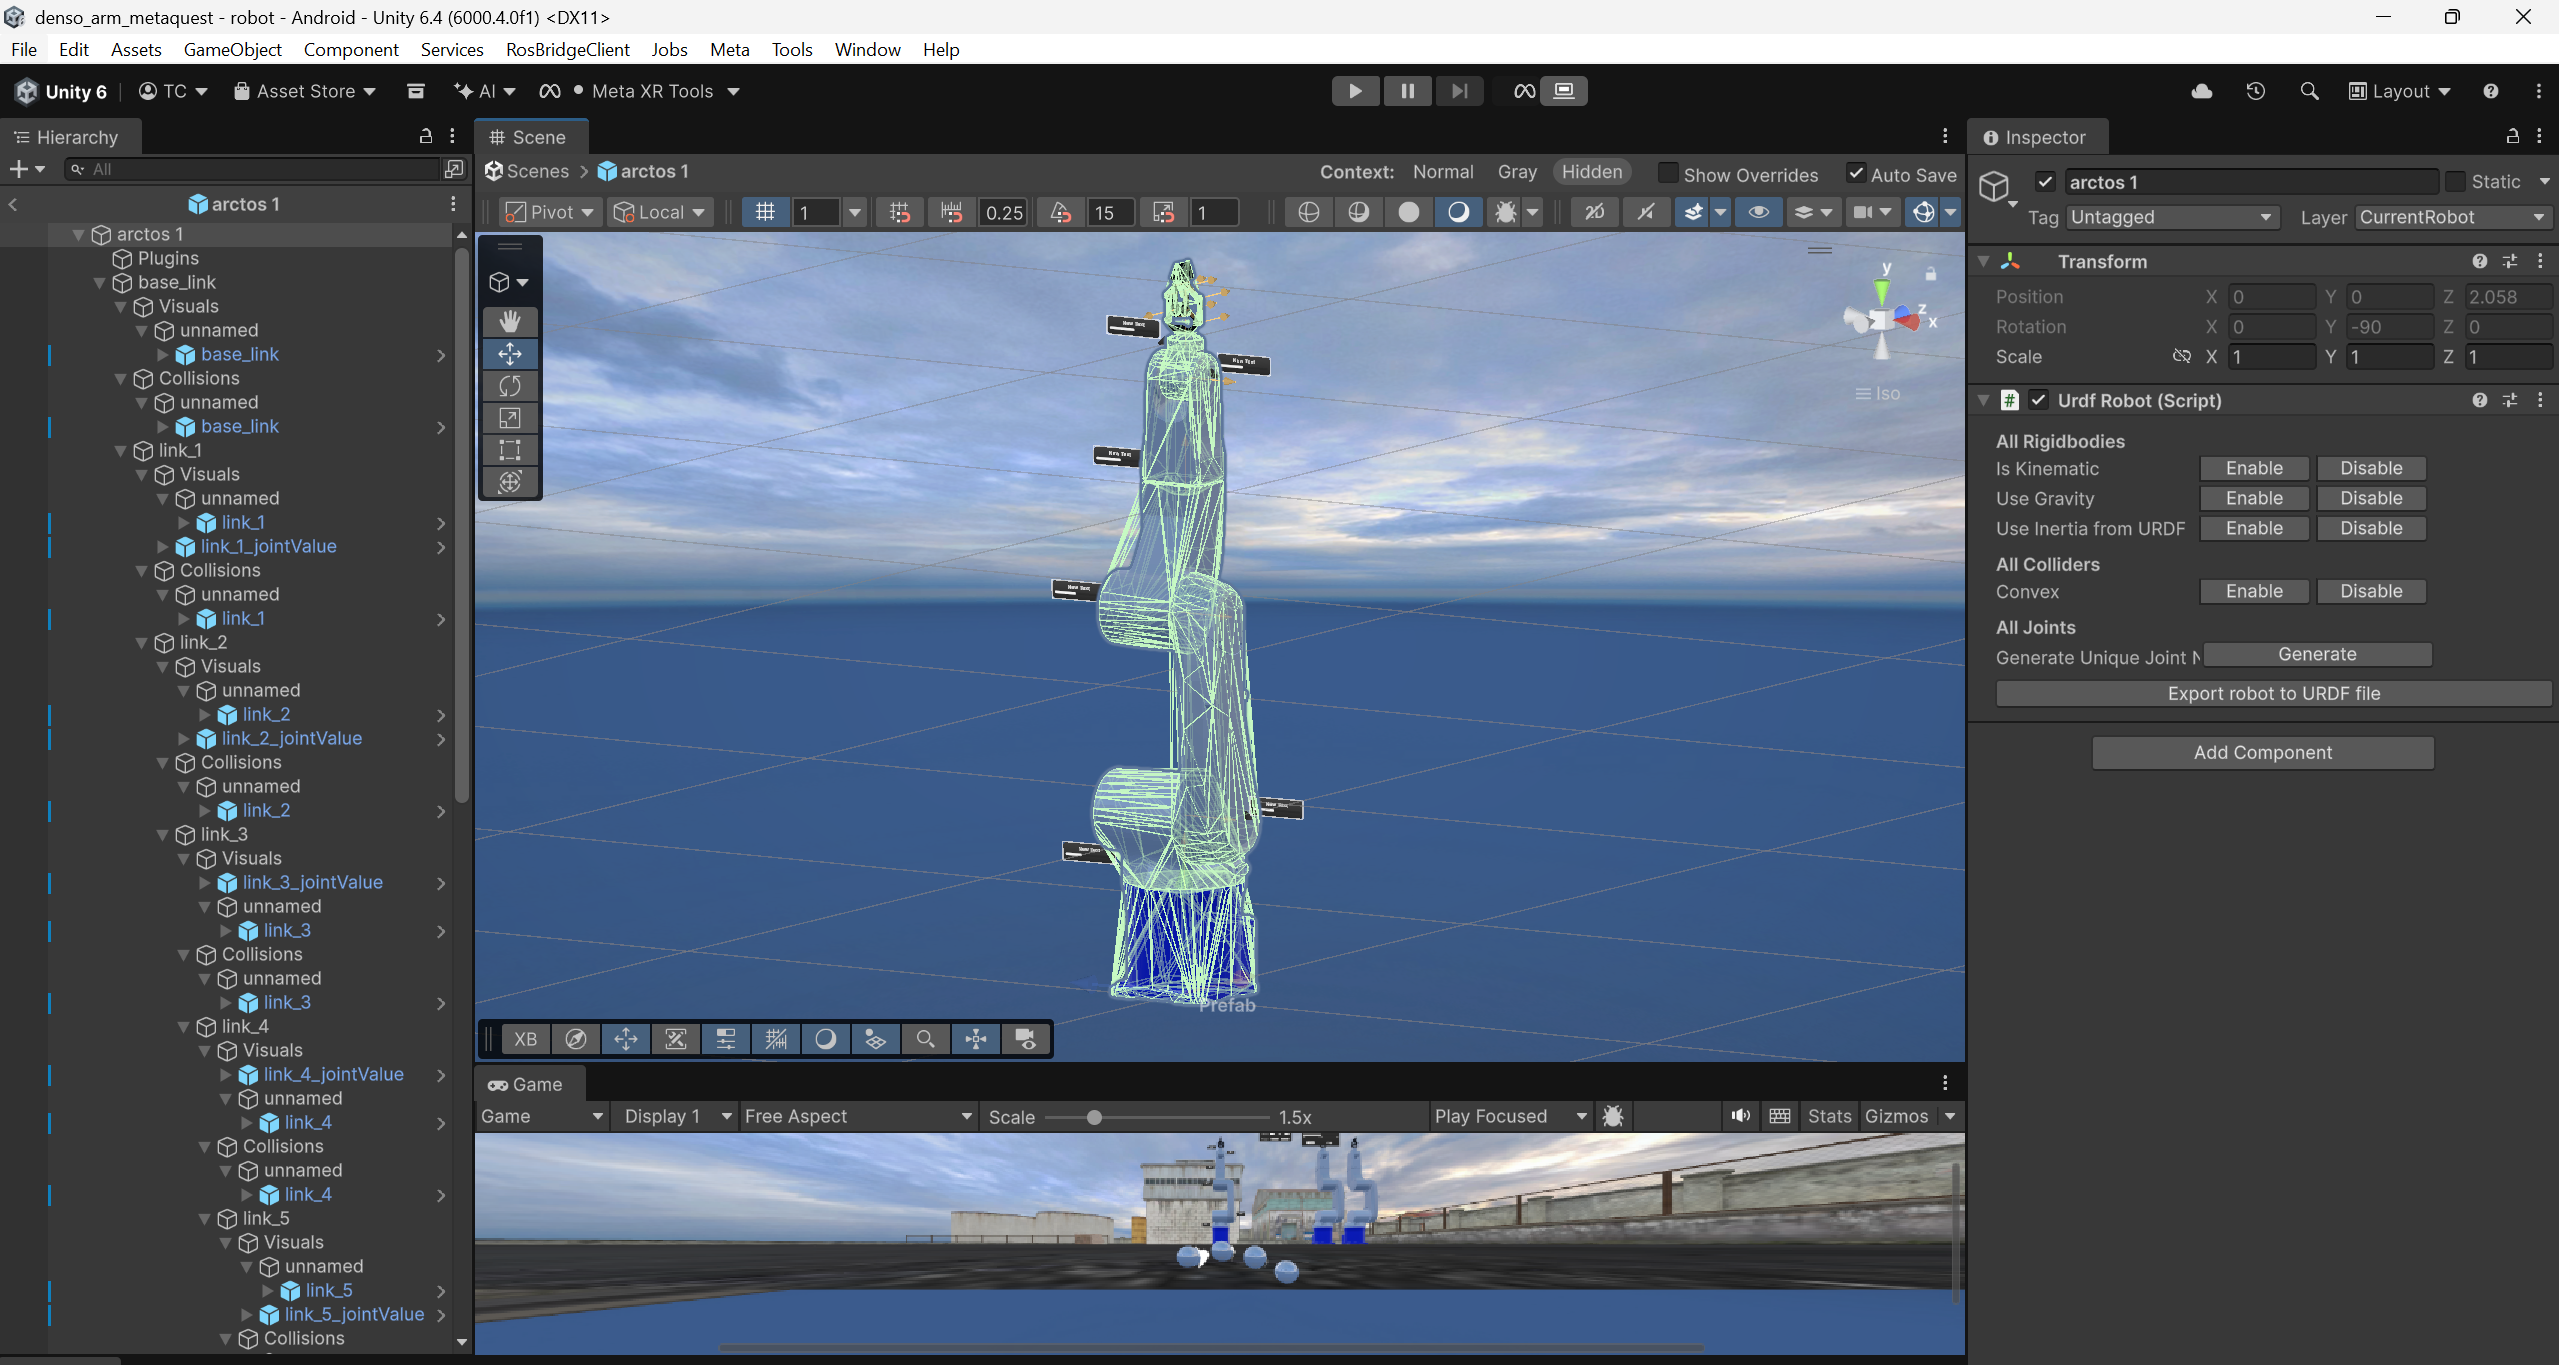
\includegraphics[width=\linewidth]{Images/Implementation/transferfromros_done.png}
        \caption{Kết quả import mô hình robot vào Unity}
    \end{subfigure}
    \caption{Quy trình chuyển mô hình robot từ ROS2 sang Unity}
    \label{fig:transfer-urdf-to-unity}
\end{figure}

\subsection{Kiến trúc phần mềm của ứng dụng VR trên Unity}

Kiến trúc phần mềm cho ứng dụng VR, tương tự cũng sẽ bao gồm hai thành phần chính: Module tương tác VR và Module giao tiếp Ros2. Module tương tác VR chính là phần "giao diện", cho phép người dùng có thể thấy, di chuyển, tương tác với các bảng điều khiển (panel), với Robot, đem lại trải nghiệm khác biệt so với việc sử dụng các công cụ phần mềm 2D, 3D trên máy tính. Module giao tiếp Ros2 đảm nhận phần giao tiếp, được xem là "cốt lõi" của ứng dụng giao tiếp và điều khiển cánh tay Robot thông qua Ros2, và cũng là module được phát triển chủ yếu của đề tài.  

% \\begin{figure}[H]
%     \\centering
%     \\includegraphics[width=0.85\\linewidth]{Images/Implementation/Control/VR_architecture.jpg}
%     \\caption{Kiến trúc tổng quan ứng dụng VR: Module giao tiếp ROS2 và Module tương tác VR}
%     \\label{fig:vr-app-architecture}
% \\end{figure}

\subsection{Module tương tác VR}

Điểm ấn tượng của module Meta XR SDK, đó là được thiết kế để nhà phát triển có thể dễ dàng bắt đầu một dự án VR/AR trên Unity với các "building block" gói gọn những tính năng thông dụng nhất để có thể sử dụng ngay. Thành phần cốt lõi nhất của một ứng dụng sử dụng Meta XR SDK là Camera Rig, với đầy đủ những tính năng như:

\begin{figure}[H]
    \centering
    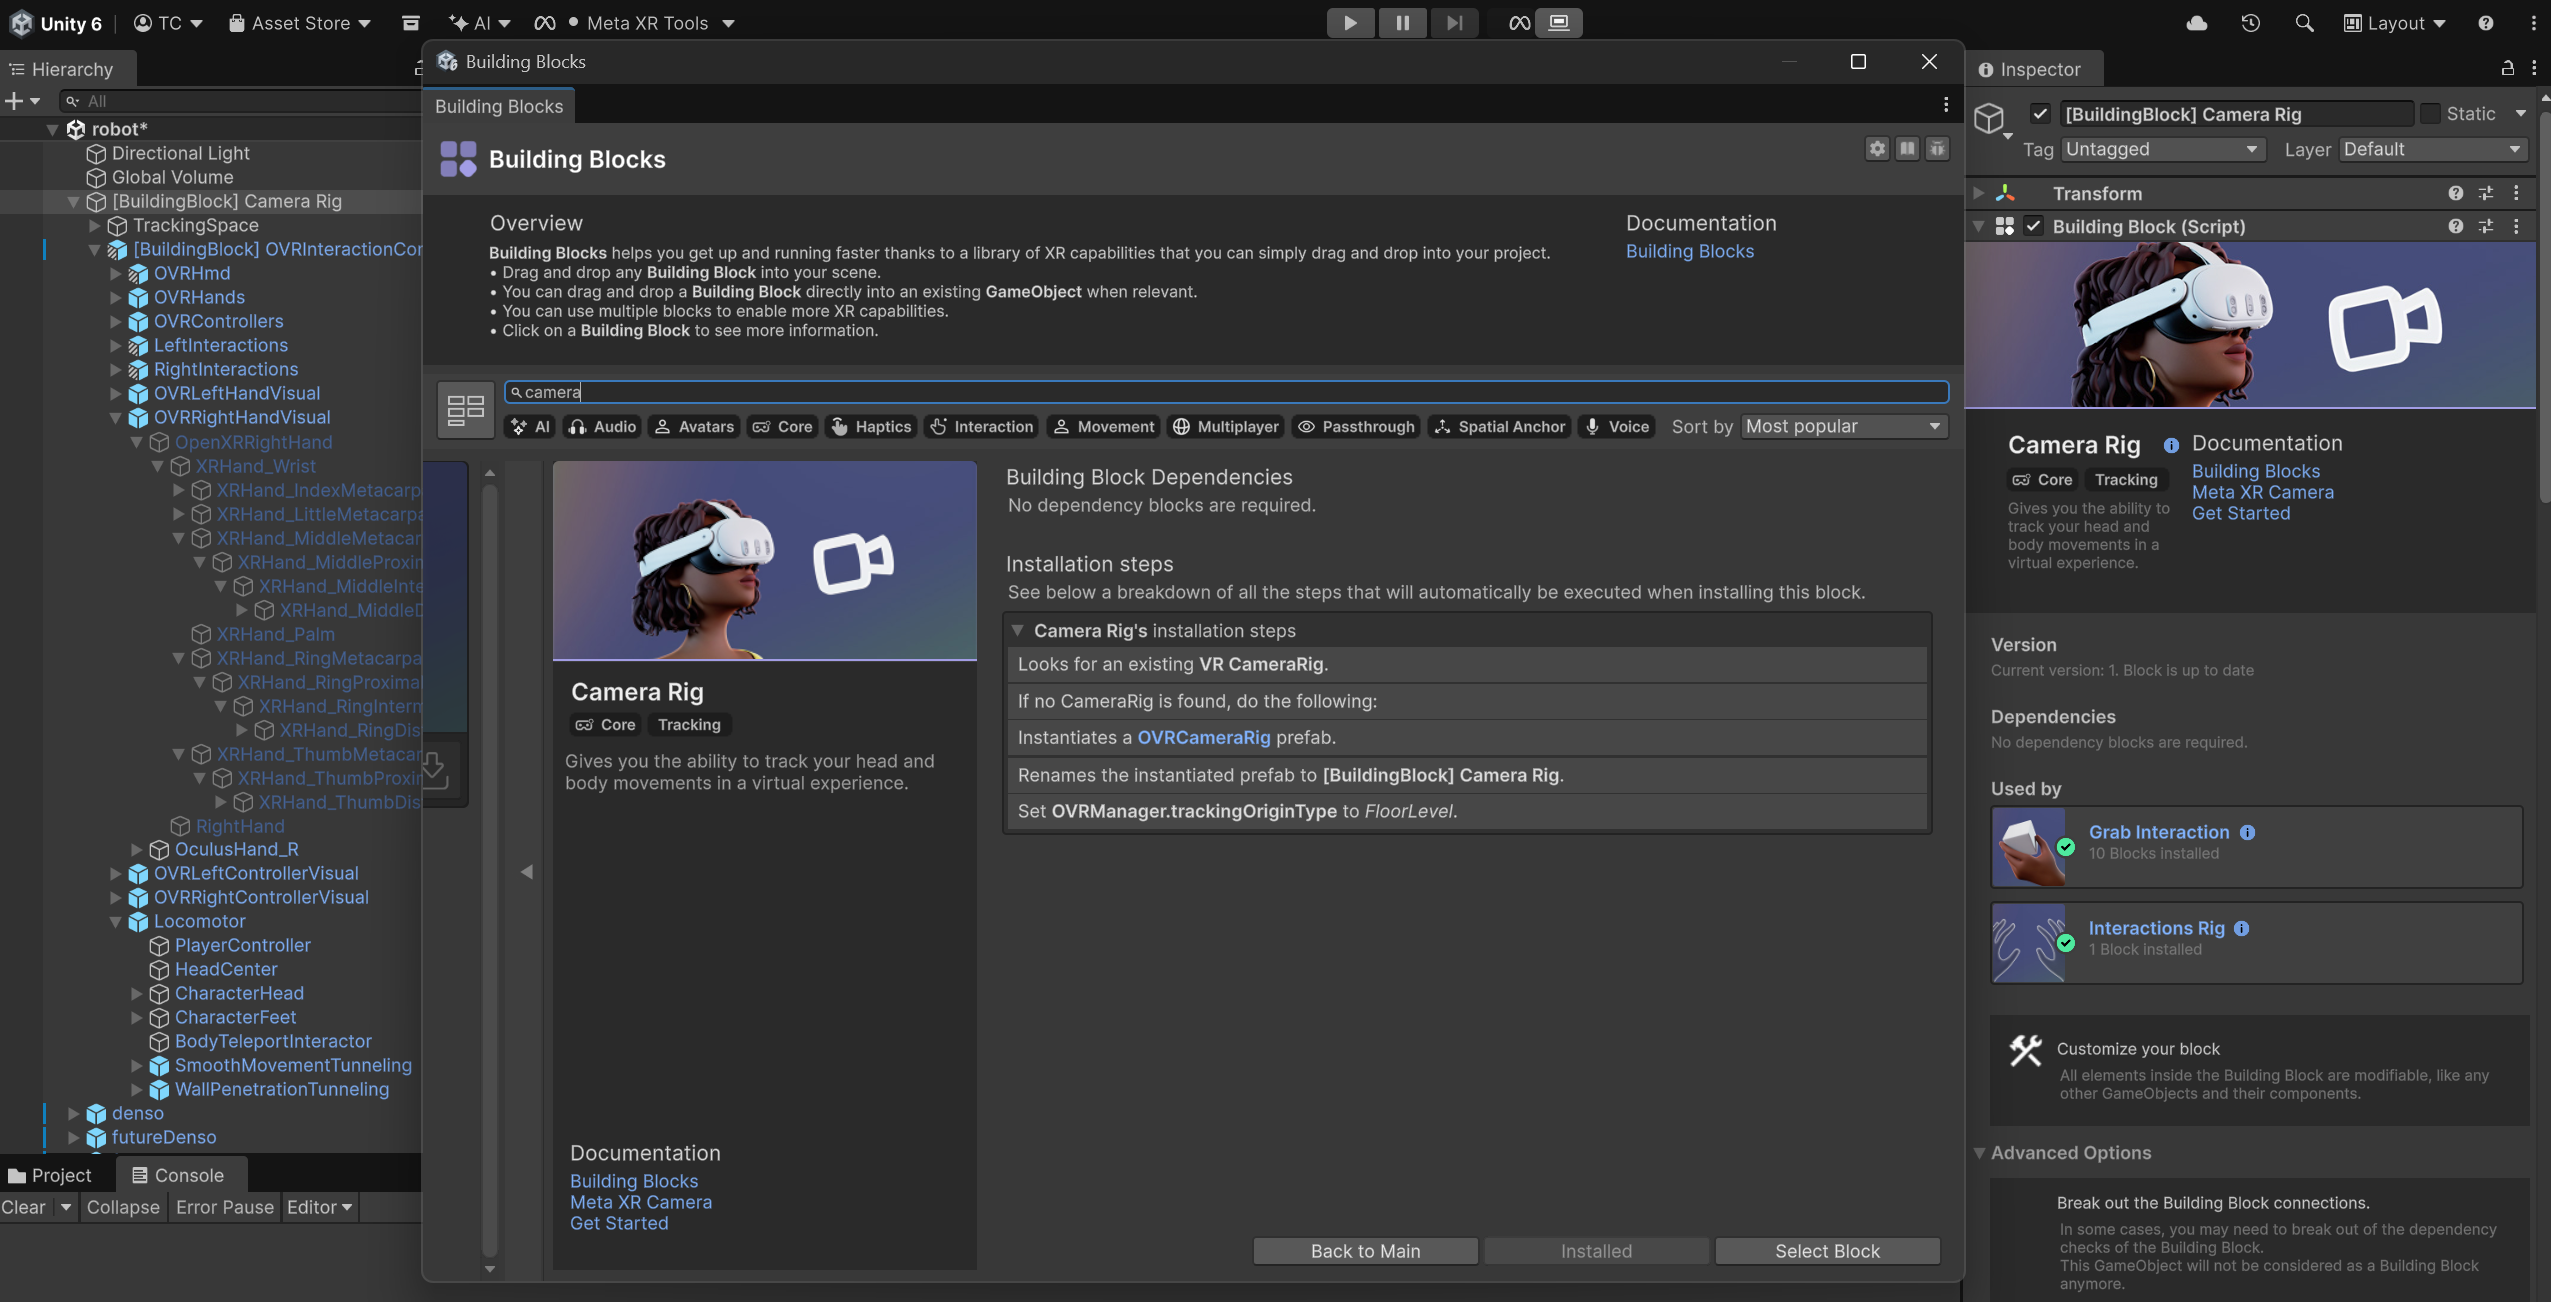
\includegraphics[width=0.7\linewidth]{Images/Implementation/camerarig.png}
    \caption{Camera Rig trong Meta XR SDK}
    \label{fig:camera-rig-meta-sdk}
\end{figure}

\begin{itemize}
    \item Giúp cho người dùng có được góc nhìn trong môi trường VR/AR, hỗ trợ head tracking, eye tracking, cho phép người dùng nhìn xung quanh, xoay đầu trong thế giới ảo
    \item Hỗ trợ di chuyển, xoay nhân vật trong môi trường ảo
    \item Hỗ trợ sử dụng tay cầm, hoặc theo dõi cử động tay và mô phỏng bàn tay trong môi trường ảo. Có thể chuyển từ dạng tay cầm sang mô phỏng bàn tay bằng cách gõ hai tay cầm lại với nhau hai lần. Ngược lại, nhấn nút trên tay cầm sẽ cho phép chuyển từ bày tay mô phỏng sang tay cầm.
    \item Là một "Interactor" giúp đem lại khả năng tương tác với vật thể có thể tương tác được (Interactable).
    \item Cho phép cấu hình nhiều thông số cho việc render hình ảnh trong úng dụng VR, đã được tối ưu với các giá trị khuyên dùng bởi Meta.
\end{itemize}

Việc tương tác được với vật thể cũng là một yếu tố quan trọng cho một ứng dụng VR. Có ba phương pháp để tương tác được hỗ trợ bởi Meta SDK, bao gồm: Poke, Ray và Grab. Các thiết lập cho từng loại tương tác có sự khác biệt đặc trưng:

\begin{itemize}
    \item \textbf{Poke Interactable}: Đây là tương tác cho phép người dùng "Nhấn" lên một đối tượng, thường là nút bấm. Poke Interactable cho phép "nhấn" bằng tay cầm, hoặc dùng ngón tay nếu sử dụng bàn tay mô phỏng. Poke Interatable yêu cầu một Clipped Plane Surface (mặt phẳng cắt) để biết được mặt phẳng mà người dùng sẽ "nhấn" lên.
    \item \textbf{Ray Interactable}: Khi một đối tượng được thêm Ray Interactable, nó cho phép người dùng có thể "trỏ" tới vật thể và tương tác với nó từ xa thông qua tay cầm, hoặc bàn tay mô phỏng. Ray Interactable thường được sử dụng cho giao diện, UI để người dùng có thể nhanh chóng thực hiện thao tác từ xa mà không cần tới gần. Ray Interactable cũng yêu cầu Clipped Plan Surface (mặt phẳng cắt) để biết giới hạn mặt phẳng được trỏ tới.
    \item \textbf{Grab Interactable}: Tương tác nắm có phần phức tạp hơn, và cũng là loại tương tác được dùng phổ biến trong ứng dụng VR. Với Grab Interactable, người dùng có thể cầm nắm vật thể, bằng tay gắp hoặc bàn tay mô phỏng, hỗ trợ nhiều kiểu nắm khác nhau và cho phép di chuyển vật thể trong không gian VR. Để sử dụng Grab Interactable, cần phải sử dụng Building block "Grab Interactable" từ Meta SDK, kèm theo định nghĩa đối tượng là một "Grabbable". Đối tượng cũng cần có "Rigid body" và "Box Collider" để người dùng có thể tác động tới đối tượng và thực hiện hành động nắm.
\end{itemize}

Các Panel điều khiển trong ứng dụng sử dụng cả 3 loại tương tác, và một mô hình 3D "Grab Future Denso Robot" sử dụng Grab Interactable cho phép người dùng tương tác và xoay từng trục của cánh tay một cách trực quan.

\subsection{Module giao tiếp Ros2}

Sơ đồ bên dưới thể hiện kiến trúc tổng quát của module giao tiếp với Ros2 thông qua Web socket. Ros connector là trung tâm của kết nối, một khi khởi tạo và kết nối thành công sẽ cho phép ứng dụng subscribe/publish tới các topic, cũng như sử dụng Service và Action theo nhu cầu. Dữ liệu truyền từ ứng dụng VR sử dụng Ros-Sharp và Ros2 cùng Ros Bridge là các chuỗi JSON theo format message thống nhất.

\subsubsection{Kết nối tới Ros2}

\begin{figure}[H]
    \centering
    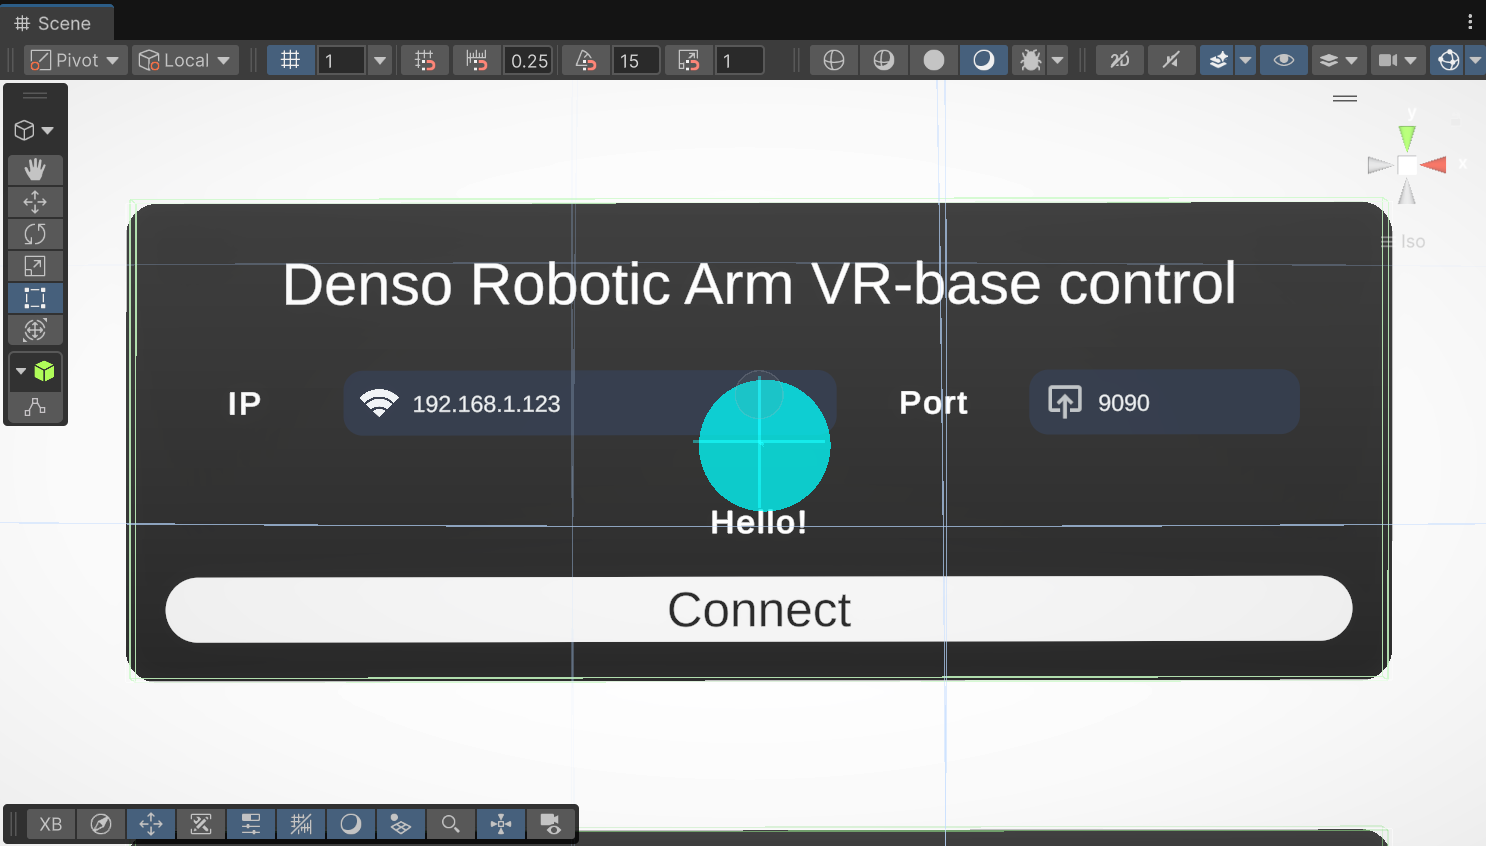
\includegraphics[width=0.75\linewidth]{Images/Implementation/connect_panel.png}
    \caption{Connect Panel và luồng kết nối tới ROS2 qua RosBridge}
    \label{fig:unity-connect-panel}
\end{figure}

Bảng điều khiển để kết nối (connect panel) là điểm khởi đầu cho ứng dụng kết nối. Tại đây, người dùng có thể tương tác với với hai TextField: IP Address và Port để điền vào địa chỉ của máy đang chạy Ros2 cùng RosBridge Server và tạo kết nối tới port đã chọn. Giá trị port ở đây sẽ là 9090, như đã cấu hình cho RosBridge Server ở phía máy PC chạy Ros2. 

Sau khi nhập địa chỉ, nhấn nút Connect để bắt đầu kết nối tới Ros2. Module "Connect to Ros2 Manager" đảm nhận việc thu thập giá trị IP và port đã định nghĩa và khởi tạo kết nối tới Ros2. Trạng thái của kết nối sẽ được hiển thị trực quan ngay trên nút kết nối. 

Khi kết nối thành công, các panel điều khiển khác sẽ hiện ra đầy đủ, cho phép người dùng tiến hành điều khiển cánh tay robot thông qua VR. Ngược lại, khi không còn sử dụng, người dùng có thể nhấn nút Disconnect để hủy kết nối tới Ros2, và các bảng điều khiển cũng sẽ tắt đi tương ứng.

\subsubsection{Theo dõi Camera với Image subscription}

Khi kết nối thành công tới PC chạy Ros2, các dịch vụ phụ thuộc vào Ros2 Connector sẽ tự động khởi chạy theo, trong đó có Compressed Image Subscriber, có nhiệm vụ subscribe vào topic hình ảnh nén (compressed image) từ Ros2. 

\begin{figure}[H]
    \centering
    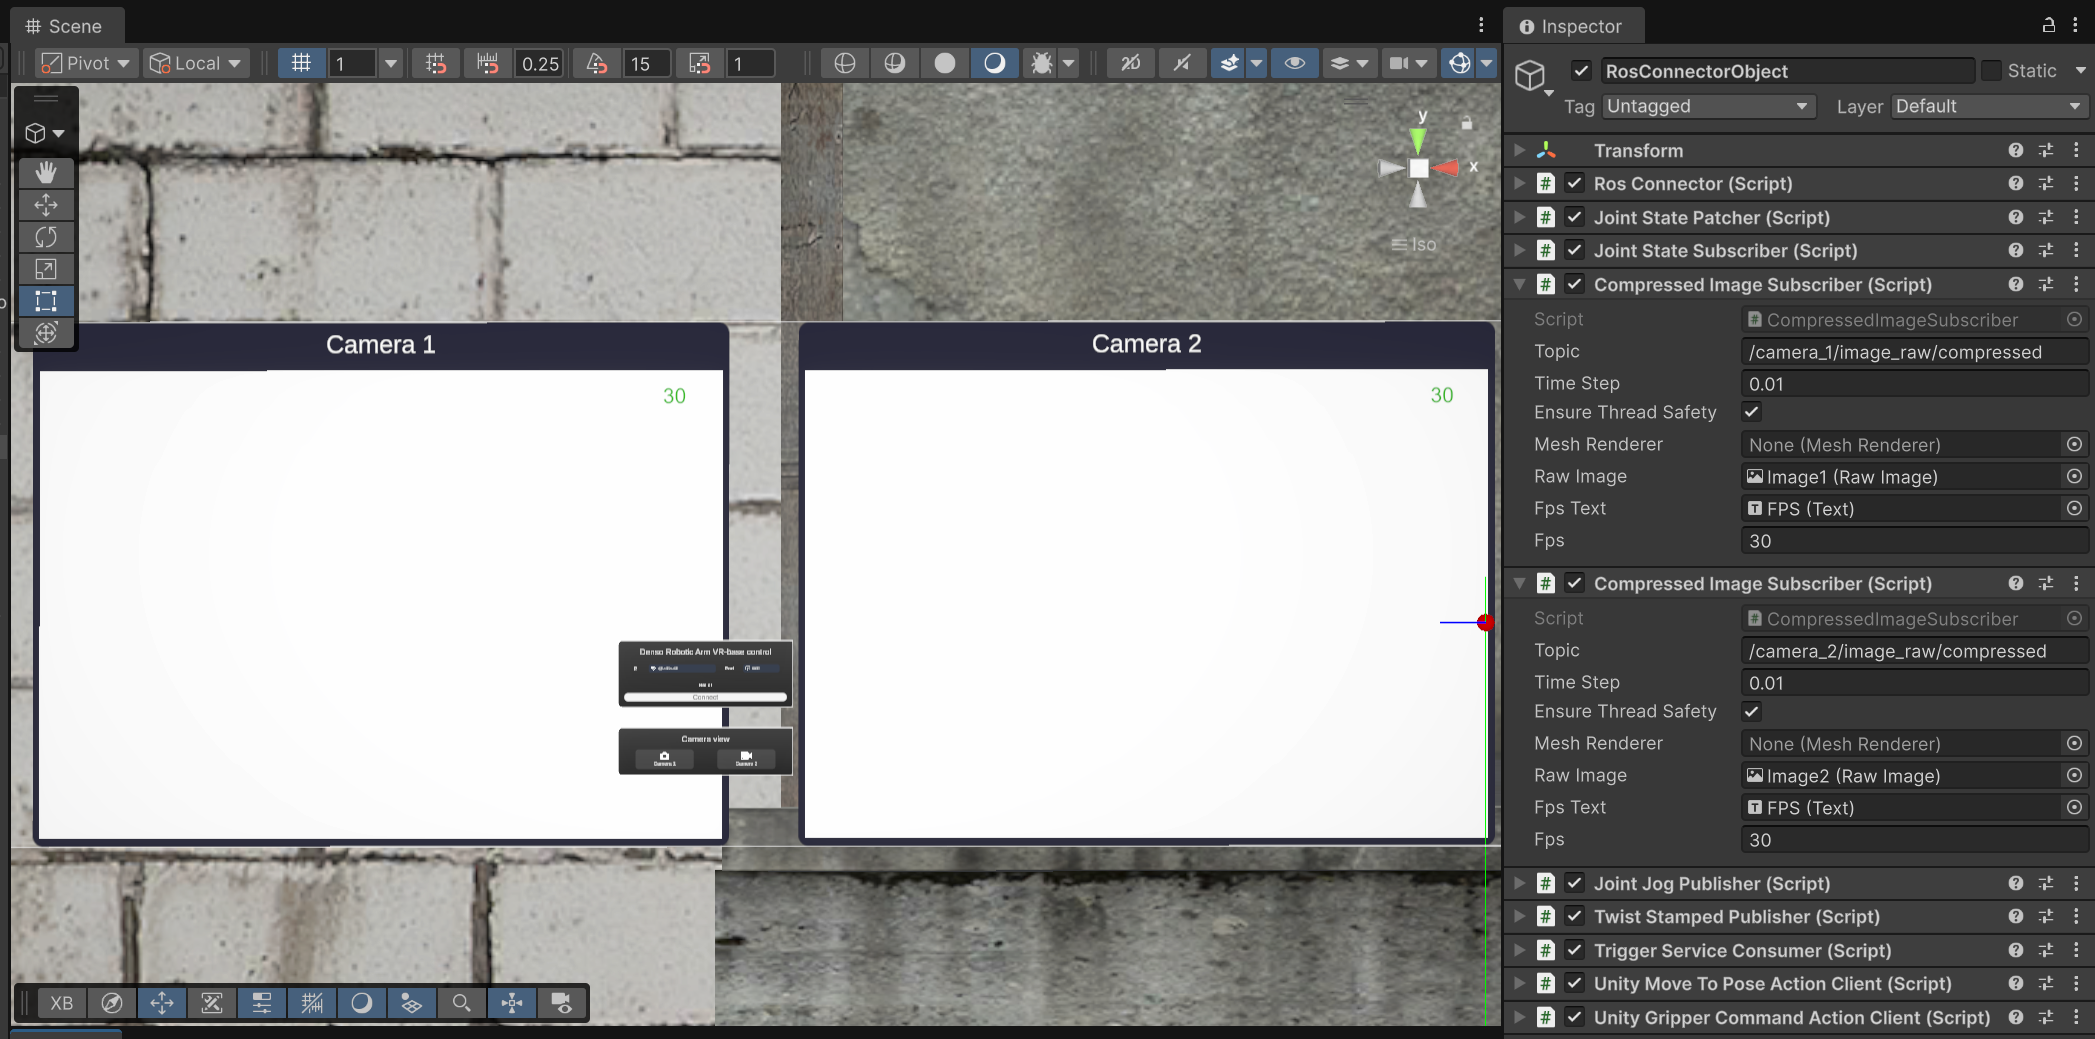
\includegraphics[width=0.72\linewidth]{Images/Implementation/image_subscriber.png}
    \caption{Cấu hình Compressed Image Subscriber trong Unity}
    \label{fig:image-subscriber-unity}
\end{figure}

Do nhu cầu sử dụng hai camera, sẽ có hai Compressed Image Subscriber được sử dụng, mỗi một subscriber truy cập tới một topic. Thuộc tính "Time Step" cho biết Subscriber sẽ xét dữ liệu mới mỗi 0.01s, hay 10ms. Khi có dữ liệu mới, hàm \lstinline[style=inlinecode]{ReceiveMessage()} của script này sẽ được gọi kèm dữ liệu ảnh. Dữ liệu ảnh được chuyển thành Texture2D ngay sau đó, và hiển thị lên "Raw Image". Ngoài ra, Script cũng hỗ trợ thu thập giá trị FPS ảnh thu được, cụ thể là một đối tượng Text ở góc phải trên của mỗi màn hình camera.

\subsubsection{Theo dõi trạng thái Robot thực tế thông qua Joint State subscription}

Để theo dõi trạng thái của cánh tay thực tế, Joint State Subscriber được sử dụng để subscribe vào topic \lstinline[style=inlinecode]{/joint\_states} nhằm theo dõi vị trí các trục robot được gửi ra từ Robot State Publisher. Joint Names là một mảng mà ta có thể ghi rõ tên của các trục cần theo dõi giá trị vị trí (hay góc) ở từng phần tử (Element). Joint State Writer của Element tương ứng sẽ được sử dụng để trực tiếp xoay trục của cánh tay robot với giá trị góc nhận được, từ đó hiện thực cơ chế đồng bộ giữa mô hình Denso Robot và trạng thái cánh tay robot thực tế được gửi ra từ Ros2. 

% \begin{figure}[H]
%     \centering
%     \includegraphics[width=0.72\linewidth]{Images/Implementation/Control/DensoHand_Read_flow.jpg}
%     \caption{Cấu hình Joint State Subscriber}
%     \label{fig:joint-state-subscriber-unity}
% \end{figure}

Đối với phần tay gắp, do đây là loại tay gắp song song (parallel gripper), nên cấu hình robot từ Ros2 sẽ chỉ có duy nhất một trục của tay gắp được truyền là trục bên phải (gripper\_gear\_right\_joint). Để tạo cơ chế điều khiển cả hai trục trái và phải của mô hình 3D trong ứng dụng VR, script đã được tùy chỉnh để hỗ trợ mirror joint (trục ánh xạ), bằng cách dùng chung tên cho phần Joint names, và phần Joint state Writer sẽ là hai trục trái và phải. 

\subsubsection{Điều khiển robot với MoveIt Servo}

Khi nói đến ứng dụng điều khiển cánh tay robot, nhu cầu đầu tiên sẽ là điều khiển từng trục của robot xoay trực tiếp. MoveIt-Servo Panel hỗ trợ nhu cầu này, bằng cách cho phép người dùng kích hoạt tính năng MoveIt-Servo từ Ros2, sau đó gửi lệnh xoay trục (JointJog) hoặc xoay tọa độ (Twist Stamped) tới MoveIt-Servo. Panel có thiết kế giao diện như sau:

\begin{figure}[H]
    \centering
    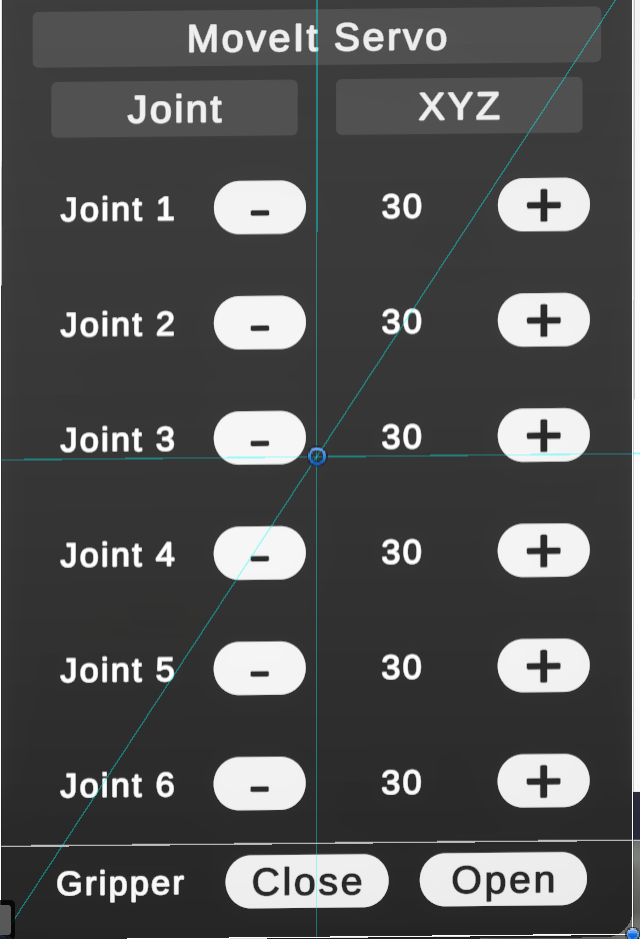
\includegraphics[width=0.72\linewidth]{Images/Implementation/moveit_servo_panel.png}
    \caption{Giao diện MoveIt-Servo Panel trong ứng dụng VR}
    \label{fig:moveit-servo-panel-unity}
\end{figure}

Đầu tiên, người dùng cần phải kích hoạt tính năng MoveIt-Servo, bằng cách gửi một Trigger Service request tới Denso MoveIt Servo node chạy trên PC Ros2. Hỗ trợ cho tính năng này, UnityServiceConsumer và TriggerServiceConsumer được xây dựng, với UnityServiceConsumer là một abstract class chung cho Serivce, và TriggerServiceConsumer cung cấp phương thức gửi Service request và nhận Service response cho một loại service (Trigger).

Service Request dạng Trigger được gửi tới Ros2 cho việc bật/tắt MoveIt-Servo là:

\begin{itemize}
    \item \textbf{Bật MoveIt-Servo:} \lstinline[style=inlinecode]{/denso_moveit_servo_node/start_servo}
    \item \textbf{Tắt MoveIt-Servo:} \lstinline[style=inlinecode]{/denso_moveit_servo_node/stop_servo}
\end{itemize}

Sau khi bật MoveIt-Servo, người dùng có thể tiếp tục thực hiện điều khiển xoay từng trục trong 6 trục (Chế độ Joint) hoặc xoay theo tọa độ (Chế độ XYZ). JointJogPublisher được dùng để publish JointJog message tới topic \lstinline[style=inlinecode]{/denso_moveit_servo_node/delta_joint_cmds}, và TwistStampedPublisher publish TwistStamped message vào topic \lstinline[style=inlinecode]{/denso_moveit_servo_node/delta_twist_cmds}. Để điều khiển, người dùng chỉ cần nhấn vào nút "+" hoặc nút "-" của từng trục để thực hiện gửi lệnh điều khiển tăng/giảm góc tới trục tương ứng, tương tự với việc thay đổi tọa độ XYZ.

Ngoài ra, ở mỗi hàng điều khiển trục, con số ở giữa cho biết giá trị góc của trục hiện tại, lấy từ nhiều "Joint State Reader" được đặt ở từng trục trong mô hình Denso Robot, để người dùng thấy được chính xác giá trị góc của robot trong quá trình điều khiển.

\subsubsection{Đóng mở Gripper với GripperCommand Action Client}

Trong MoveIt-Servo panel, ngoài tính năng điều khiển bằng MoveIt-Servo, ta còn có hai nút nhấn để thực hiện đóng/ mở tay gắp. Đối với controller của tay gắp được hiện thực ở phía Ros2 (denso\_hand\_controller - loại GripperActionController), do đây là loại controller đơn giản và cách điều khiển không cần quá phức tạp, đề tài chủ trương giao tiếp trực tiếp với Action Server của controller cho tay gắp, thông qua việc tạo Action client loại GripperCommand.

Trước khi hiện thực GripperCommand Action Client, ta cần định nghĩa class Action phù hợp trong Unity. Package Ros-Sharp hỗ trợ điều này thông qua tính năng Generate Action trong RosBridgeClient -> Auto Generate Action -> Single Action, và trỏ tới file action tương ứng:

\begin{figure}[H]
    \centering
    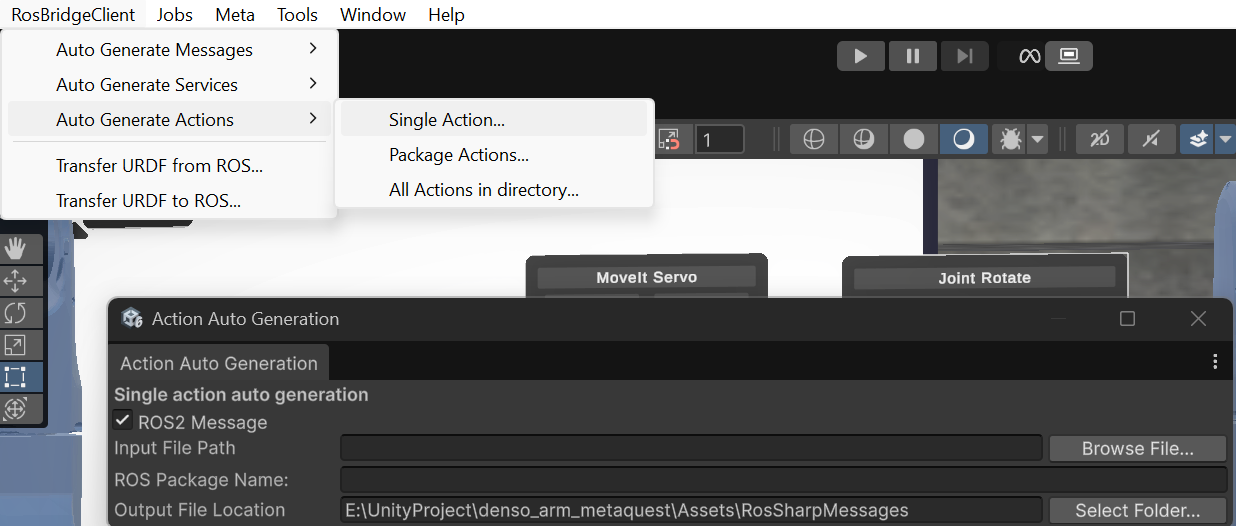
\includegraphics[width=0.75\linewidth]{Images/Implementation/generate_action.png}
    \caption{Tạo Action class trong Ros-Sharp từ file action của ROS2}
    \label{fig:generate-action-rossharp}
\end{figure}

Ros-Sharp sẽ tự động generate cho GripperCommand bảy class cho Action này, bao gồm:

\begin{enumerate}
    \item GripperCommandAction
    \item GripperCommandActionFeedback
    \item GripperCommandActionGoal
    \item GripperCommandActionResult
    \item GripperCommandFeedback
    \item GripperCommandGoal
    \item GripperCommandResult
\end{enumerate}

Tiếp đến, class GripperCommandActionClient được hiện thực, kế thừa từ class ActionClient với toàn bộ bảy class của Action GripperCommand được xây dựng, cung cấp những API cơ bản như \lstinline[style=inlinecode]{SetActionGoal(), OnFeedbackReceived(), OnResultReceived()} để gửi Goal, theo dõi feedback và sau cùng là nhận result, như một Action client cơ bản của Ros2.

Dựa trên class GripperCommandActionClient, UnityGripperCommandActionClient kế thừa MonoBehavior để phù hợp trong môi trường Unity, khởi tạo chính thức một object GripperCommandActionClient để có thể gửi lệnh đóng hoặc mở Gripper, đồng thời theo dõi feedback và result ở hàm \lstinline[style=inlinecode]{Update()} của Unity.

\begin{figure}[H]
    \centering
    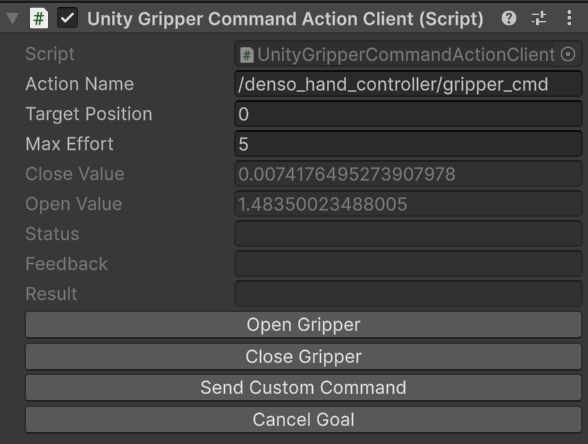
\includegraphics[width=0.75\linewidth]{Images/Implementation/unitygrippercommand.png}
    \caption{Hiện thực UnityGripperCommandActionClient}
    \label{fig:unity-gripper-command-client}
\end{figure}

\subsubsection{Điều khiển robot với MoveToPose Action Client}

MoveToPose là một custom action, dành riêng cho Denso Remote Control Action Server được hiện thực ở phần Ros2, nhằm mục tiêu gửi lệnh điều khiển robot xoay tới vị trí mong muốn thông qua giá trị góc trục hoặc tọa độ XYZ. Vì là một custom action, ta buộc phải import bộ action này vào Unity bằng tính năng Generate Action, tương tự như với Gripper Command. Bộ file được sinh ra sẽ bao gồm:

\begin{enumerate}
    \item MoveToPoseAction
    \item MoveToPoseActionFeedback
    \item MoveToPoseActionGoal
    \item MoveToPoseActionResult
    \item MoveToPoseFeedback
    \item MoveToPoseGoal
    \item MoveToPoseResult
\end{enumerate}

Class MoveToPoseActionClient được hiện thực kế thừa class ActionClient cùng bảy class của MoveToPose phía trên, chung nhiệm vụ cung cấp các API cơ bản để có thể gửi Goal, nhận feedback và result. Trên lớp MoveToPoseActionClient, UnityMoveToPoseActionClient là class được sử dụng chính: tạo object MoveToPoseActionClient nhằm tạo goal, gửi goal và liên tục lấy các kết quả. 

Điểm quan trọng trong hiện thực của MoveToPose Action Client, đó là cho phép tạo goal bằng danh sách các Joint và cả goal bằng tọa độ XYZ, tuy nhiên cơ chế điều khiển bằng tọa độ chưa có độ tin cậy tốt, bởi một giá trị tọa độ có thể có rất nhiều giá trị trục có thể thỏa mãn vị trí đó (động học nghịch), dẫn tới robot có thể được MoveIt2 planning và execute với "Pose" - hay dáng của robot không đúng như mong đợi. Cơ chế điều khiển bằng tọa độ XYZ hiện tại cần nhiều thời gian để nghiên cứu hơn, do đó chưa áp dụng cho ứng dụng điều khiển hiện tại.

Vì giới hạn trên, cơ chế điều khiển thông qua giá trị 6 trục Robot được sử dụng chủ yếu. Đối với cơ chế này, ứng dụng cung cấp hai phương thức điều khiển: Xoay trục bằng bảng điều khiển và tương tác với cánh tay để xoay.

\textbf{Xoay Robot với bảng điều khiển}

Cách thức "Xoay robot với bảng điều khiển" lấy cảm hứng dựa theo ứng dụng Rviz trên Ros2, khi người dùng được phép sử dụng các thanh ngang để xoay mô hình robot tương lai "Goal State" và xem xét hình dáng, trạng thái của cánh tay robot, trước khi thực hiện Planning và Execute. Đối với cách thức này, người dùng sẽ nhấn chọn nút Joint Rotate trên bảng điều khiển để chuyển sang mode điều khiển bằng cách xoay các slider. Các slider sẽ hiện ra, cùng với một bản sao mô hình 3D của robot Denso, gọi là "Future Denso Robot". Bản sao robot này được điều khiển hoàn toàn bởi Joint Rotate Panel, tức giá trị của slider sẽ tương ứng với giá trị của mỗi trục cánh tay. 

\begin{figure}[H]
    \centering
    \begin{subfigure}{0.48\linewidth}
        \centering
        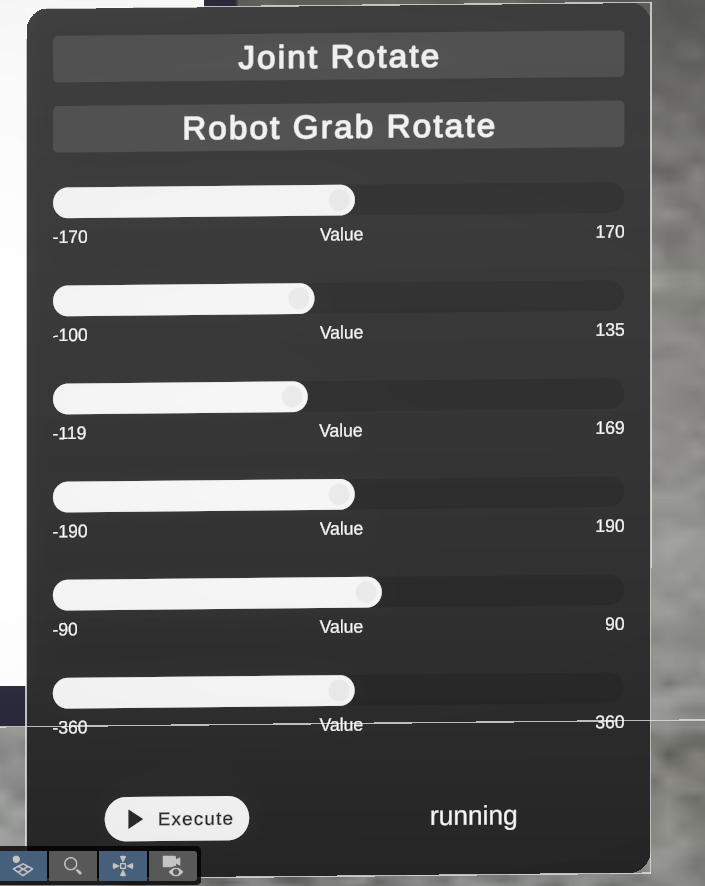
\includegraphics[width=\linewidth]{Images/Implementation/jointrotate.png}
        \caption{Joint Rotate Panel}
    \end{subfigure}
    \hfill
    \begin{subfigure}{0.48\linewidth}
        \centering
        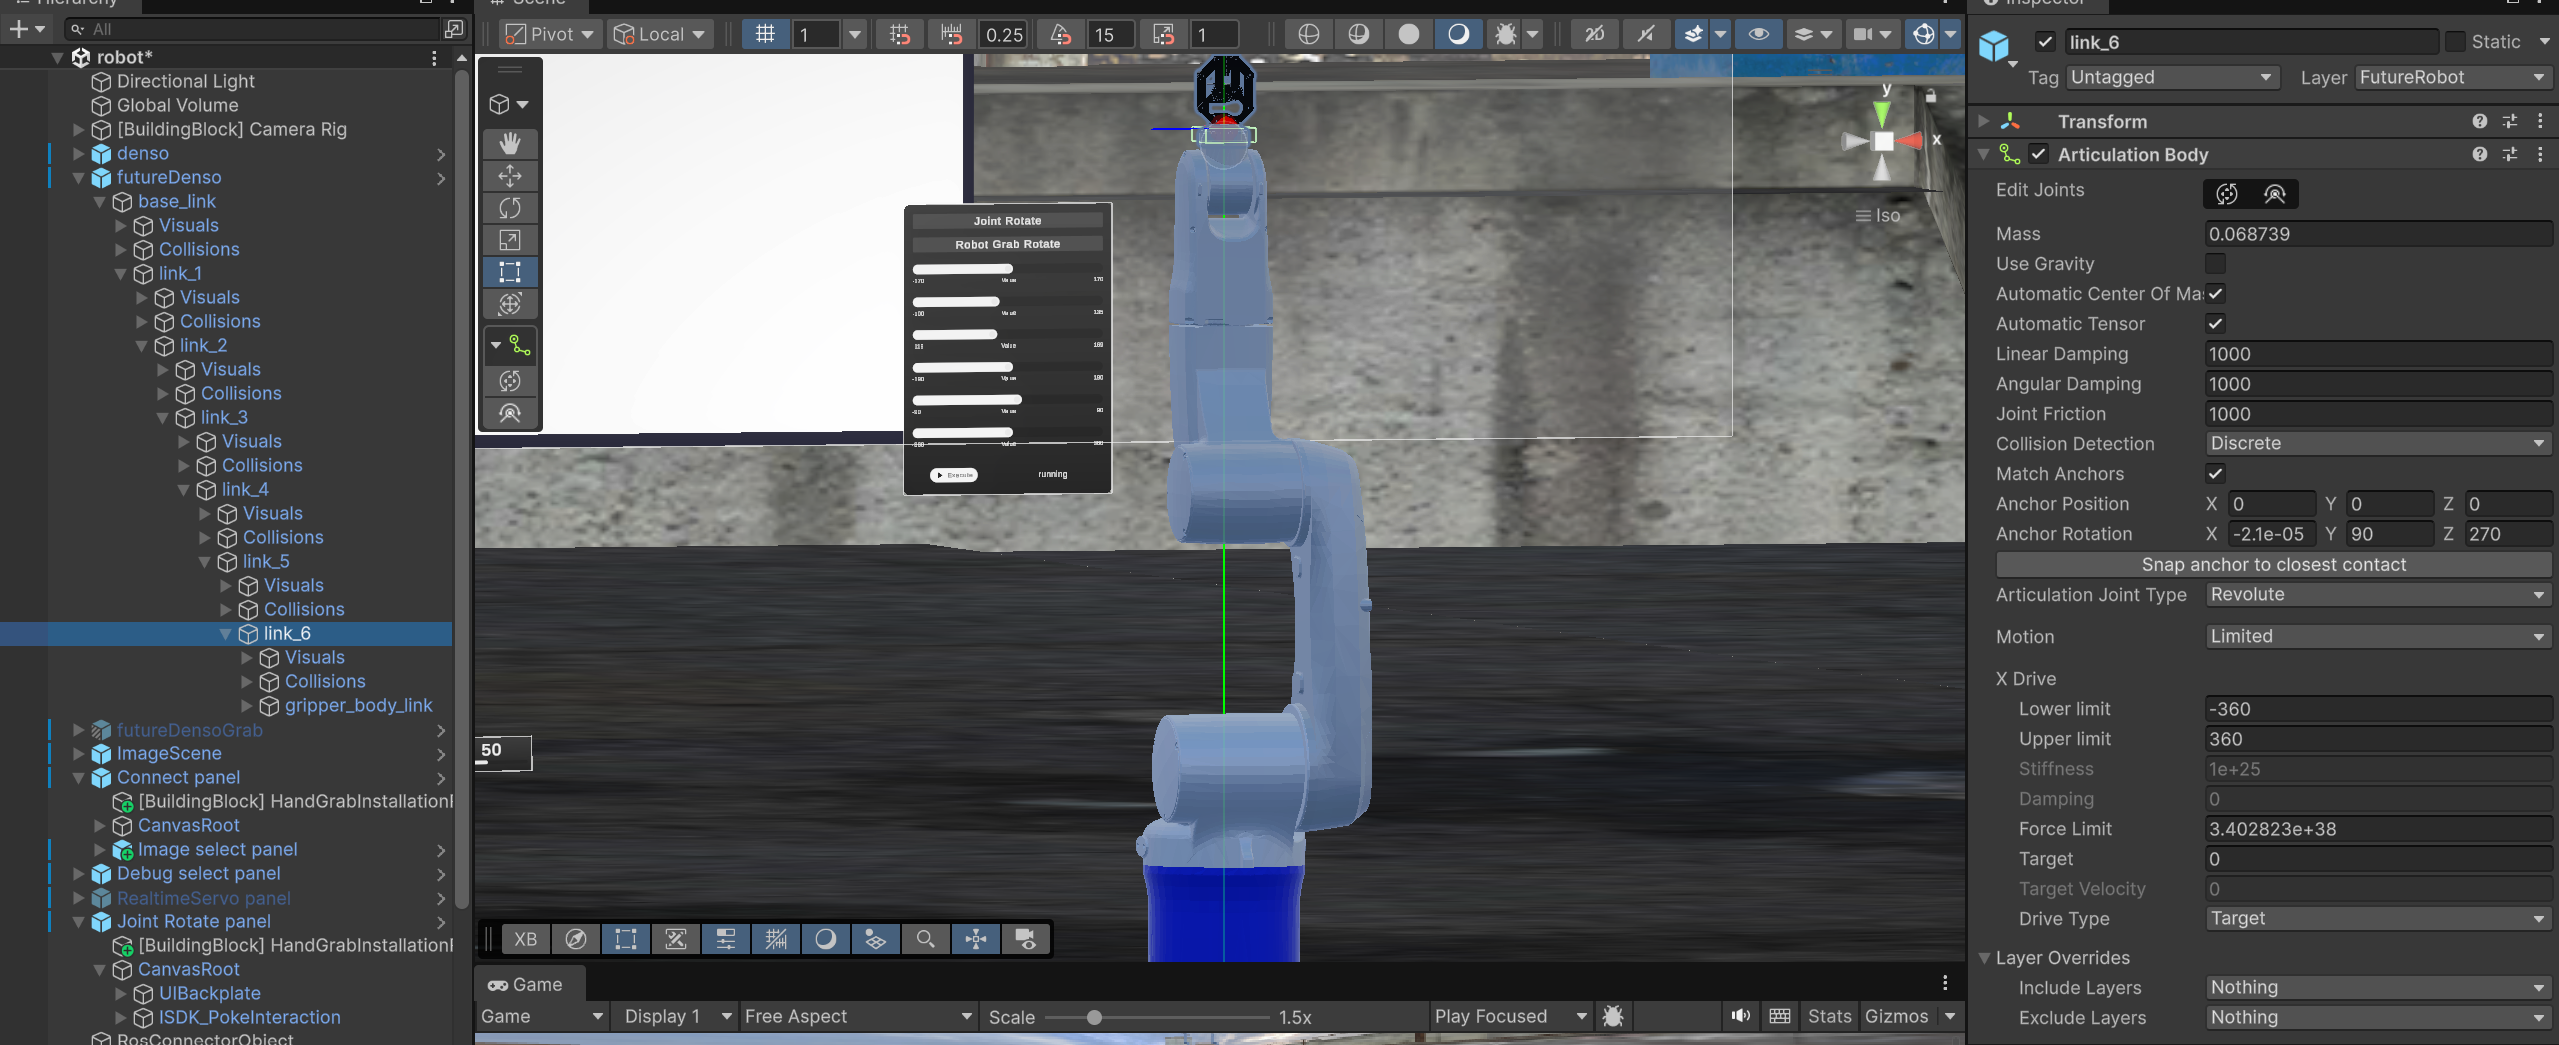
\includegraphics[width=\linewidth]{Images/Implementation/futuredenso_articulation.png}
        \caption{Future Denso Robot với Articulation Body}
    \end{subfigure}
    \caption{Điều khiển robot bằng bảng điều khiển và mô hình Future Denso Robot}
    \label{fig:joint-rotate-and-future-robot}
\end{figure}

Để đảm bảo mô hình 3D Future Denso Robot xoay mượt và ổn định, đề tài sử dụng các Articulation Body cho các trục thay vì chỉ sử dụng bộ Rigid Body + Hinge Joint để mô tả một khớp xoay tròn, kèm theo giới hạn xoay để tránh trường hợp xoay quá giá trị cho phép ở từng trục.

Sau khi đã xoay robot tới vị trí mong muốn bằng slider, nhấn nút Execute sẽ lần lượt thực hiện các bước sau:

\begin{itemize}
    \item Các giá trị góc ở từng slider được thu thập và tạo thành một List chứa giá trị góc mong muốn cho từng trục
    \item Tạo MoveToPose Goal với danh sách các trục, usePose = false.
    \item Goal được gửi tới thiết bị Ros2 thông qua UnityMoveToPoseActionClient
\end{itemize}

Khi Action Goal của MoveToPose được gửi, Action Server ở phía Ros2 sẽ nhận Goal, kiểm tra tính hợp lệ của lệnh và thực hiện Planning + Execute cánh tay tương ứng bằng MoveIt2. Trong quá trình xoay cánh tay, trạng thái của cánh tay sẽ luôn được cập nhật liên tục nhờ hoạt động của Joint State Subscriber, từ đó điều khiển mô hình chính - "Denso robot" xoay tương ứng, cho biết chính xác trạng thái thực tế của cánh tay. Quá trình Execute hoàn tất khi MoveIt2 đưa cánh tay tới vị trí tương đồng như vị trí cánh tay đã chỉnh thông qua cách bảng điều khiển bằng Slider.

\textbf{Xoay Robot bằng cách tương tác với mô hình}

Đây là cách điều khiển trực quan hơn so với việc sử dụng Slider, cho phép người dùng thật sự tương tác với model cánh tay robot. Để kích hoạt chức năng này, người dùng bấm vào nút Robot Grab Rotate để chuyển sang cách điều khiển tương tác mô hình. Giao diện của bảng điều khiển sẽ chuyển sang như hình dưới:

\begin{figure}[H]
    \centering
    \begin{subfigure}{0.48\linewidth}
        \centering
        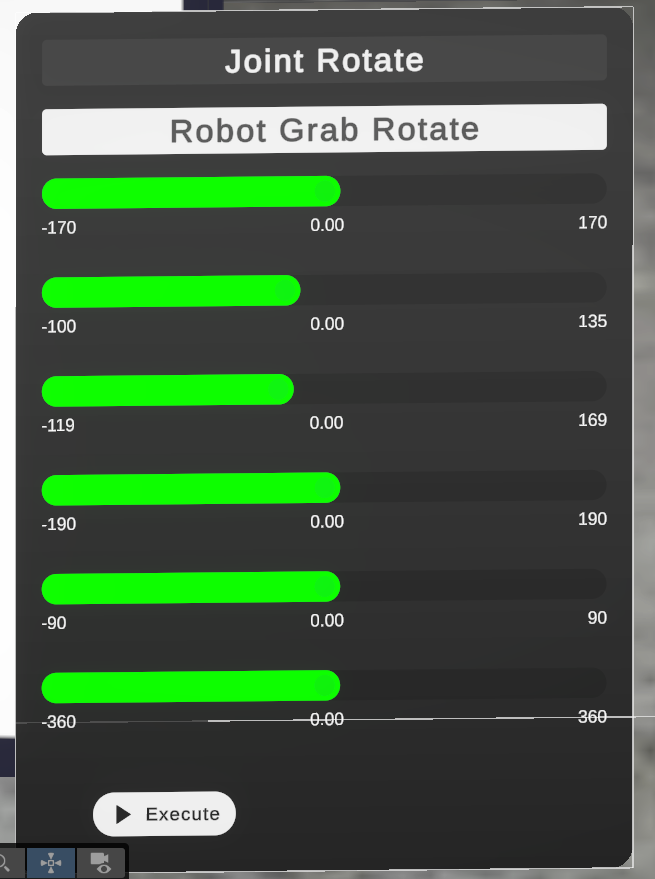
\includegraphics[width=\linewidth]{Images/Implementation/robotgrabrotate.png}
        \caption{Giao diện Robot Grab Rotate}
    \end{subfigure}
    \hfill
    \begin{subfigure}{0.48\linewidth}
        \centering
        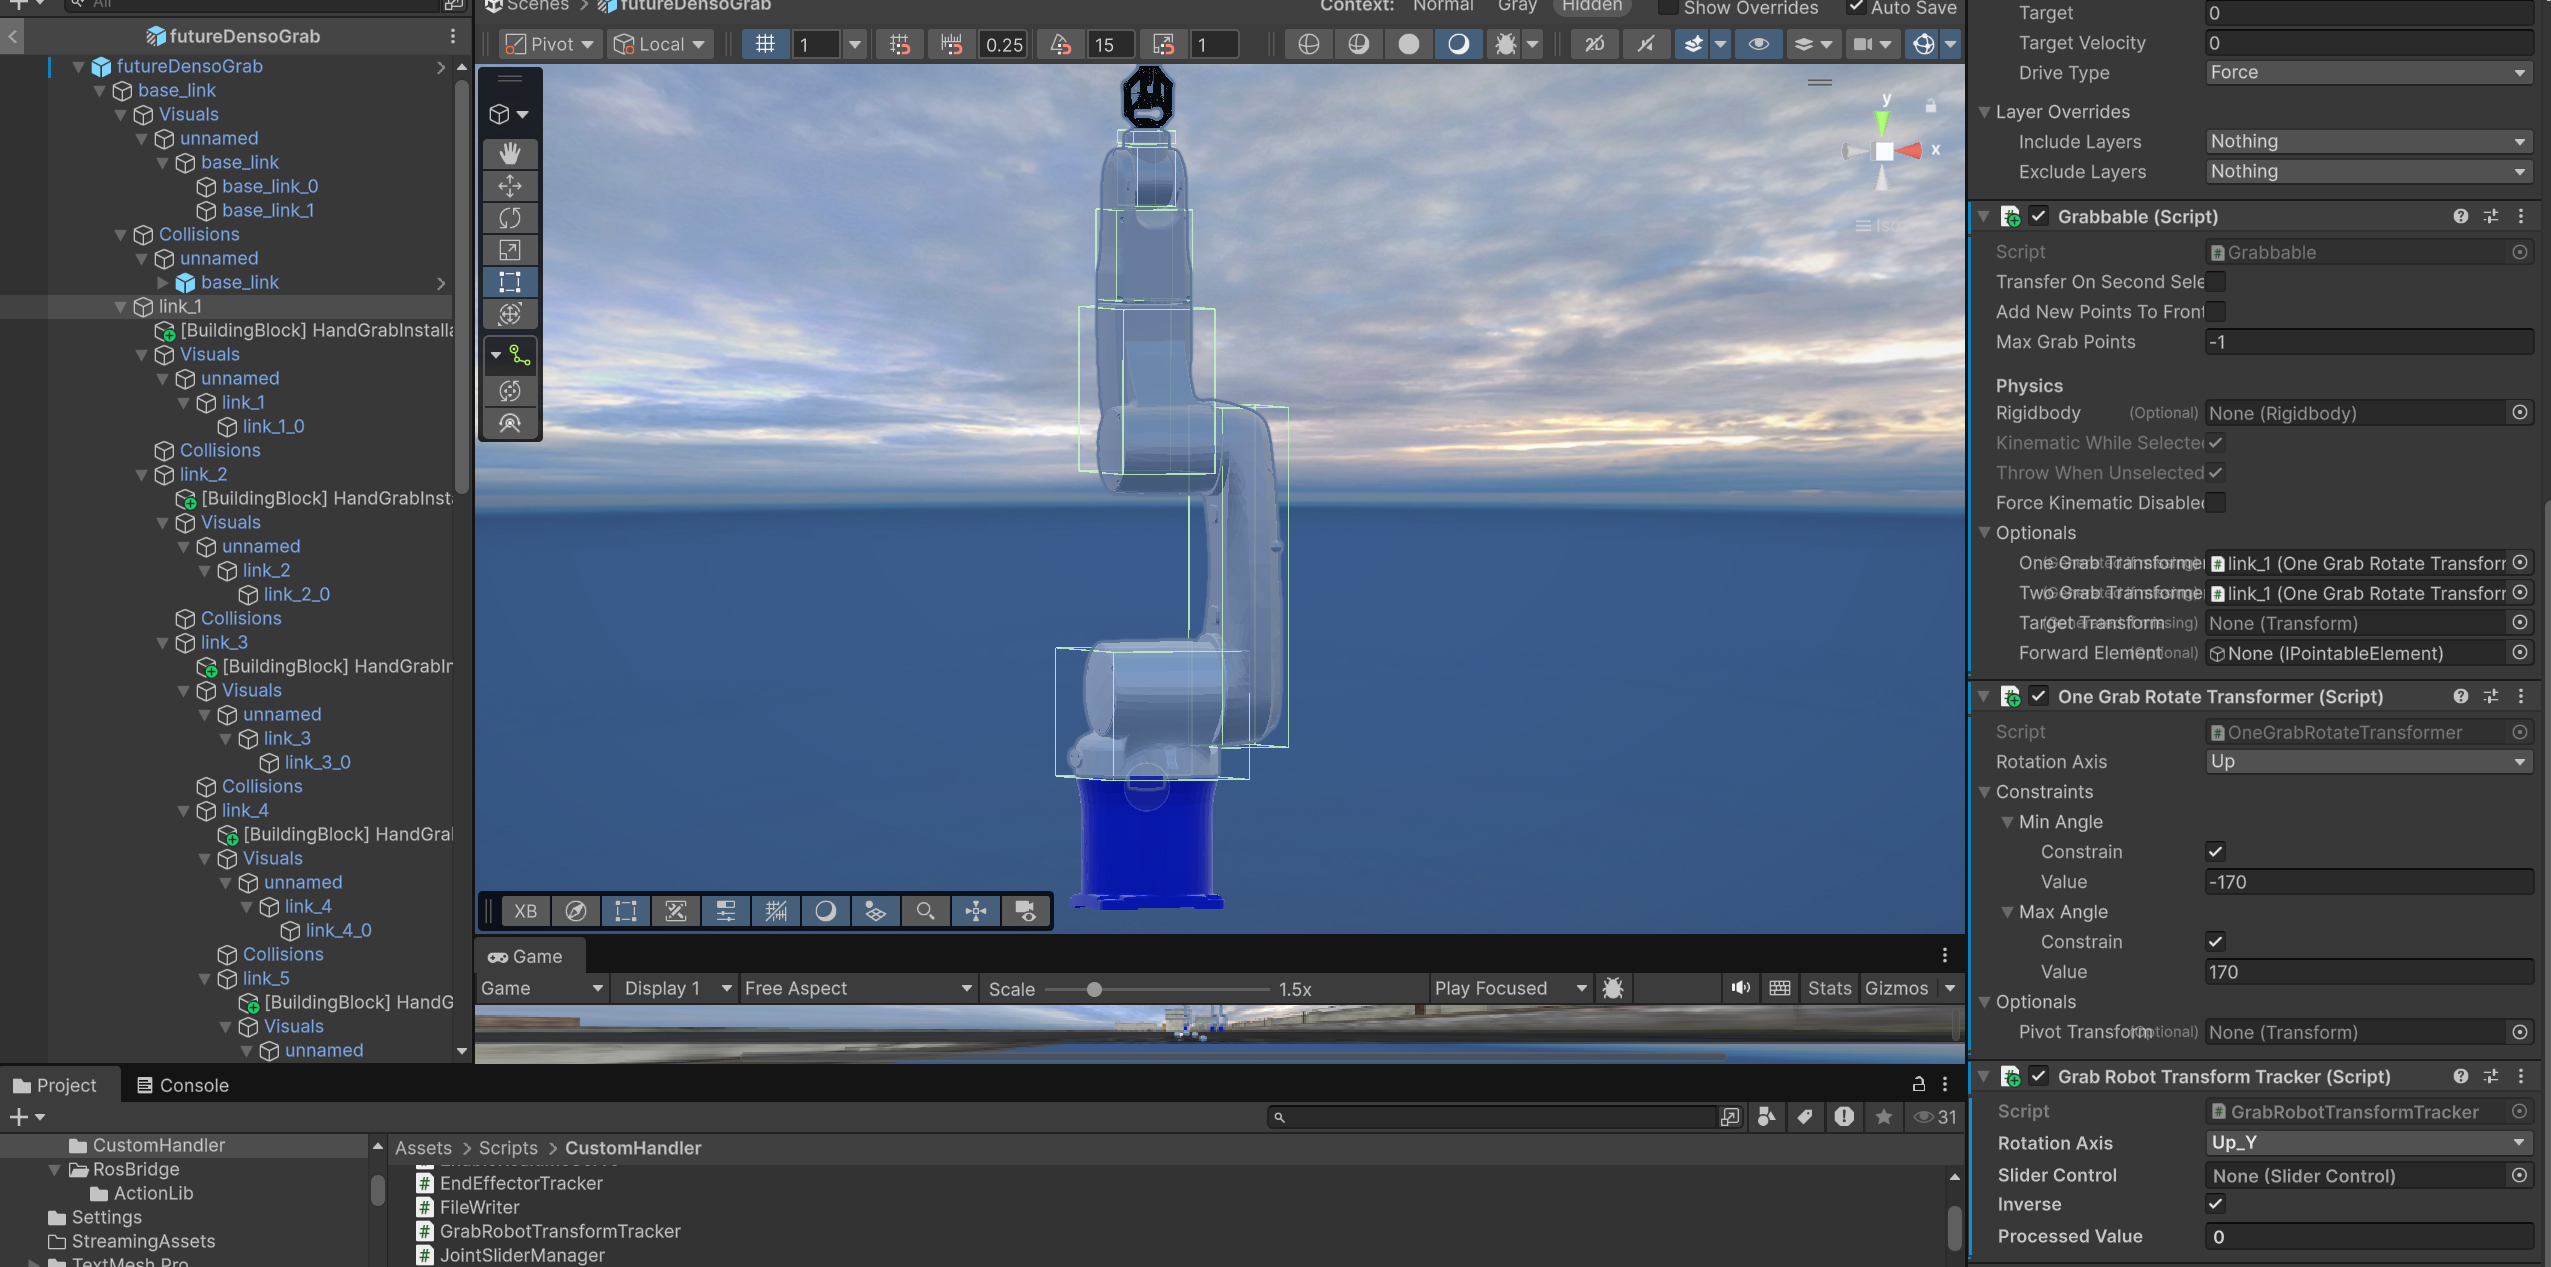
\includegraphics[width=\linewidth]{Images/Implementation/robotgrabrotate_transformer.png}
        \caption{Thiết lập OneGrabRotateTransformer}
    \end{subfigure}
    \caption{Điều khiển robot bằng tương tác nắm trực tiếp trên mô hình}
    \label{fig:robot-grab-rotate}
\end{figure}

Ở chế độ này, một mô hình 3D tương lai của robot cũng xuất hiện, cùng bộ slider mới, tuy nhiên các slider này không thể tương tác được - giá trị của nó sẽ phụ thuộc vào trạng thái của mô hình 3D "Grab Future Denso Robot". 

Về phía "Grab Future Denso Robot", ở mỗi trục sẽ được điều chỉnh để trở thành một "Grab Interactable" object, để cho phép người dùng có thể xoay từng trục bằng thao tác nắm của tay cầm hoặc bàn tay mô phỏng. OneGrabRotateTransformer được sử dụng để đảm bảo rằng khi thực hiện thao tác "grab", các trục robot chỉ có thể xoay (Rotate) quanh một trục cố định, với giới hạn min-max, tránh trường hợp người dùng cầm nắm quá tự do khiến trục bị tách rời khỏi cánh tay, hoặc trục bị xoay vượt quá ngưỡng cho phép.

Giá trị rotate của từng trục được thu thập và hiển thị lên slider để người dùng theo dõi. Khi đã xoay các trục tới vị trí mong muốn, người dùng có thể nhấn nút Execute để gửi giá trị các trục đó tới Ros2 và điều khiển cánh tay thực tế tới vị trí như yêu cầu.




